\documentclass[9pt]{beamer}
\usepackage[utf8]{inputenc}

% Theme options
\usetheme{Warsaw}
\setbeamertemplate{blocks}[rounded]
\useoutertheme{shadow}
\useinnertheme{circles}

% Packages
\usepackage{graphicx}
\usepackage{amsmath}
\usepackage{amssymb}
\usepackage{hyperref}
\usepackage{xcolor}
\usepackage{tikz}
\usetikzlibrary{tikzmark,positioning}
\usepackage{pdfpages}	% To import PDF page
\usepackage{siunitx}
\usepackage{mhchem}
\usepackage{booktabs}
\usepackage{multicol}

% Some redifinition
\makeatletter
\def\mathcolor#1#{\@mathcolor{#1}}
\def\@mathcolor#1#2#3{%
  \protect\leavevmode
  \begingroup
    \color#1{#2}#3%
  \endgroup
}
\makeatother

% Ontario Tech Colours
\definecolor{ForestGreen}{cmyk}{0.83,0.21,1,0.08}
\definecolor{ONTech-dark-blue}{cmyk}{1,0.58,0.09,0.46}
\definecolor{ONTech-light-blue}{cmyk}{1,0.31,0,0}
\definecolor{ONTech-orange}{cmyk}{0,0.70,1,0}
\definecolor{ONTech-dark-bluey}{cmyk}{0.9,0.11,0.13,0.20}
\definecolor{ONTech-cool-grey}{cmyk}{0.20,0.14,0.12,0.40}
\definecolor{ONTech-dark-grey}{cmyk}{0.45,0.25,0.16,0.59}
\definecolor{ONTech-navy}{cmyk}{1,0.75,0.50,0.50}

% Palette Modifications
\setbeamercolor{palette primary}{bg=ONTech-orange,fg=white}
\setbeamercolor{palette secondary}{bg=ONTech-dark-blue,fg=white}
\setbeamercolor{palette tertiary}{bg=ONTech-light-blue,fg=white}
\setbeamercolor{palette quaternary}{bg=ONTech-dark-blue,fg=white}
\setbeamercolor{structure}{fg=ONTech-dark-blue} % itemize, enumerate, etc
\setbeamercolor{section in toc}{fg=ONTech-dark-bluey} % TOC sections
\setbeamercolor{section in head/foot}{bg=ONTech-navy,fg=white} % Headings
\setbeamercolor{subsection in head/foot}{bg=ONTech-light-blue,fg=white} % Headings

%% Add slide numbers in navigation bar
%\addtobeamertemplate{navigation symbols}{}{%
%    \usebeamerfont{footline}%
%    \usebeamercolor[fg]{footline}%
%    \hspace{1em}%
%    \insertframenumber/\inserttotalframenumber
%}

% Footnote without number
\newcommand\blfootnote[1]{%
  \begingroup
  \renewcommand\thefootnote{}\footnote{#1}%
  \addtocounter{footnote}{-1}%
  \endgroup
}

% Math vector and matrix commands
\renewcommand{\vec}[1]{\ensuremath{\boldsymbol{#1}}}
\newcommand{\mtx}[1]{\ensuremath{\boldsymbol{#1}}}

% For no navigation symbols on section start pages
\AtBeginSection[]{%
  \begingroup
  \setbeamertemplate{navigation symbols}{}
  \begin{frame}
  \frametitle{Outline}
  \tableofcontents[currentsection]
  \end{frame}
  \endgroup
}

% For footnote mark in braces.
\renewcommand*{\thefootnote}{(\arabic{footnote})}

\title[PhD Candidacy Examination]{Thermochemical Equilibrium for Multiphysics Simulations of Nuclear Materials}
\subtitle{Development of the Corrosion Modelling Application Yellowjacket}
\author{Parikshit Bajpai}
\institute{\footnotesize{ Supervisor: Prof. Markus H.A. Piro}}
\date{\scriptsize{PhD Candidacy Examination \\ \today}}

\begin{document}

\begingroup
\setbeamertemplate{navigation symbols}{}
{
\setbeamercolor{background canvas}{bg=}

\includepdf{Cover/Backup.pdf}
}
\endgroup

%\frame{\titlepage}

%\frame{\tableofcontents}

%\begingroup
%\setbeamertemplate{navigation symbols}{}
%\begin{frame}
%\frametitle{Outline}
%\tableofcontents
%\end{frame}
%\endgroup

%\section{Introduction}
\subsection{Overview of the Beamer Class}
\frame
{
  \frametitle{Features of the Beamer Class}

  \begin{itemize}
  \item<1-> Normal LaTeX class.
  \item<2-> Easy overlays.
  \item<3-> No external programs needed.      
  \end{itemize}
}
%\section{Goals of Research}
\subsection{Impetus}
\frame{
	\frametitle{Role of Thermochemistry}
	\only<1> {\begin{figure}
	\centering
	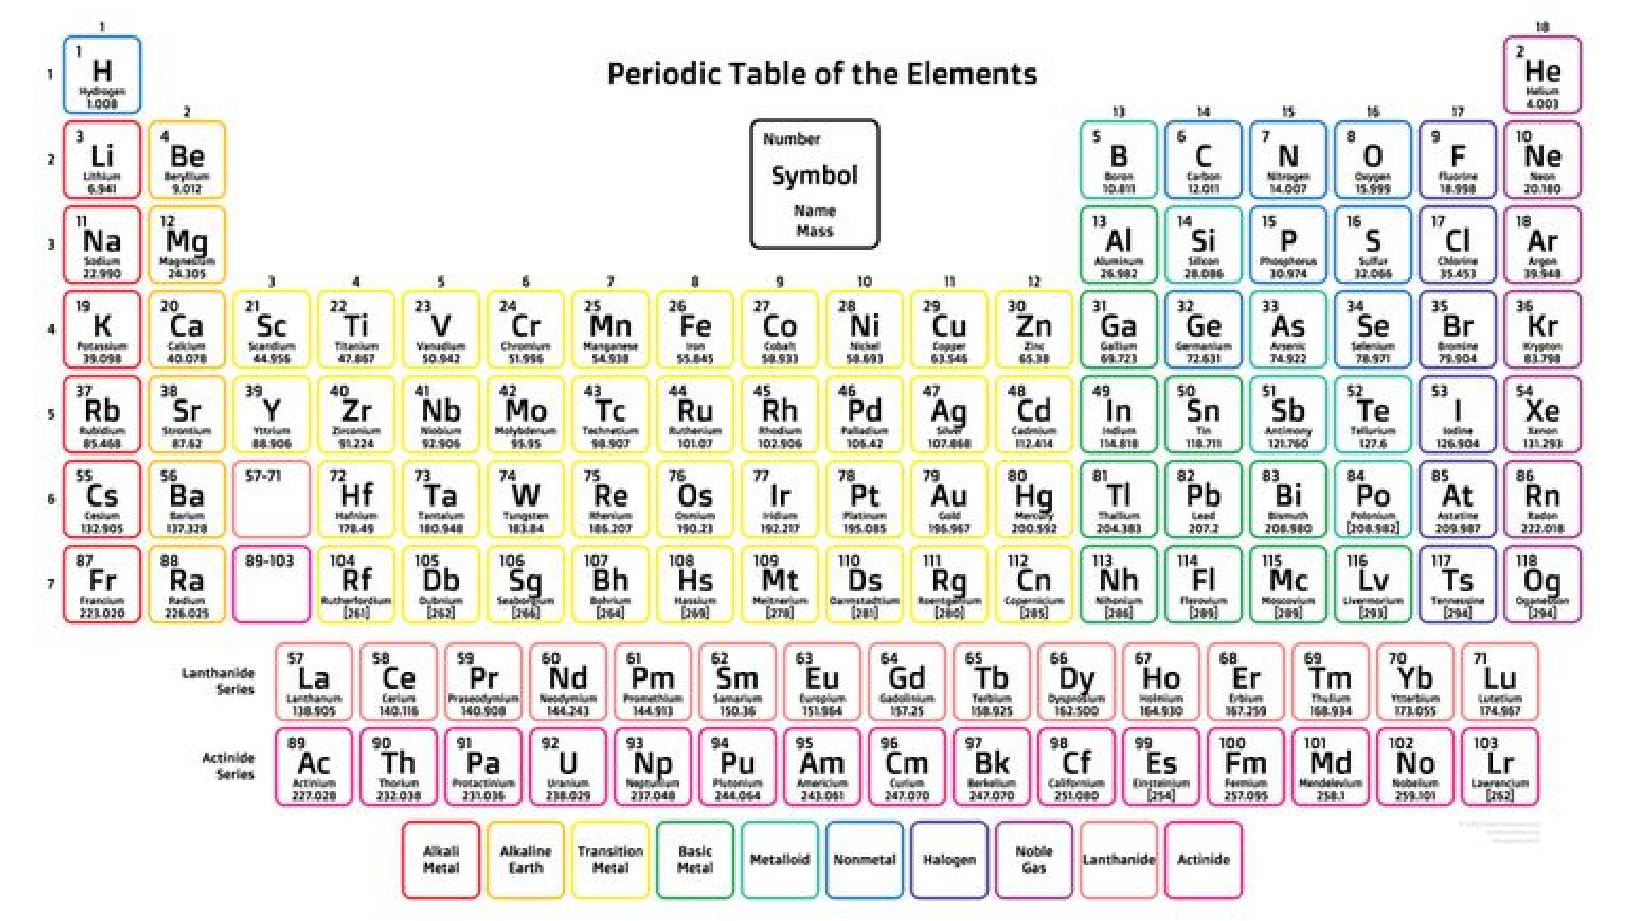
\includegraphics[width=\textwidth]{Figures/PT.pdf}
	\end{figure}
	}
	
	\only<2> {\begin{figure}
	\centering
	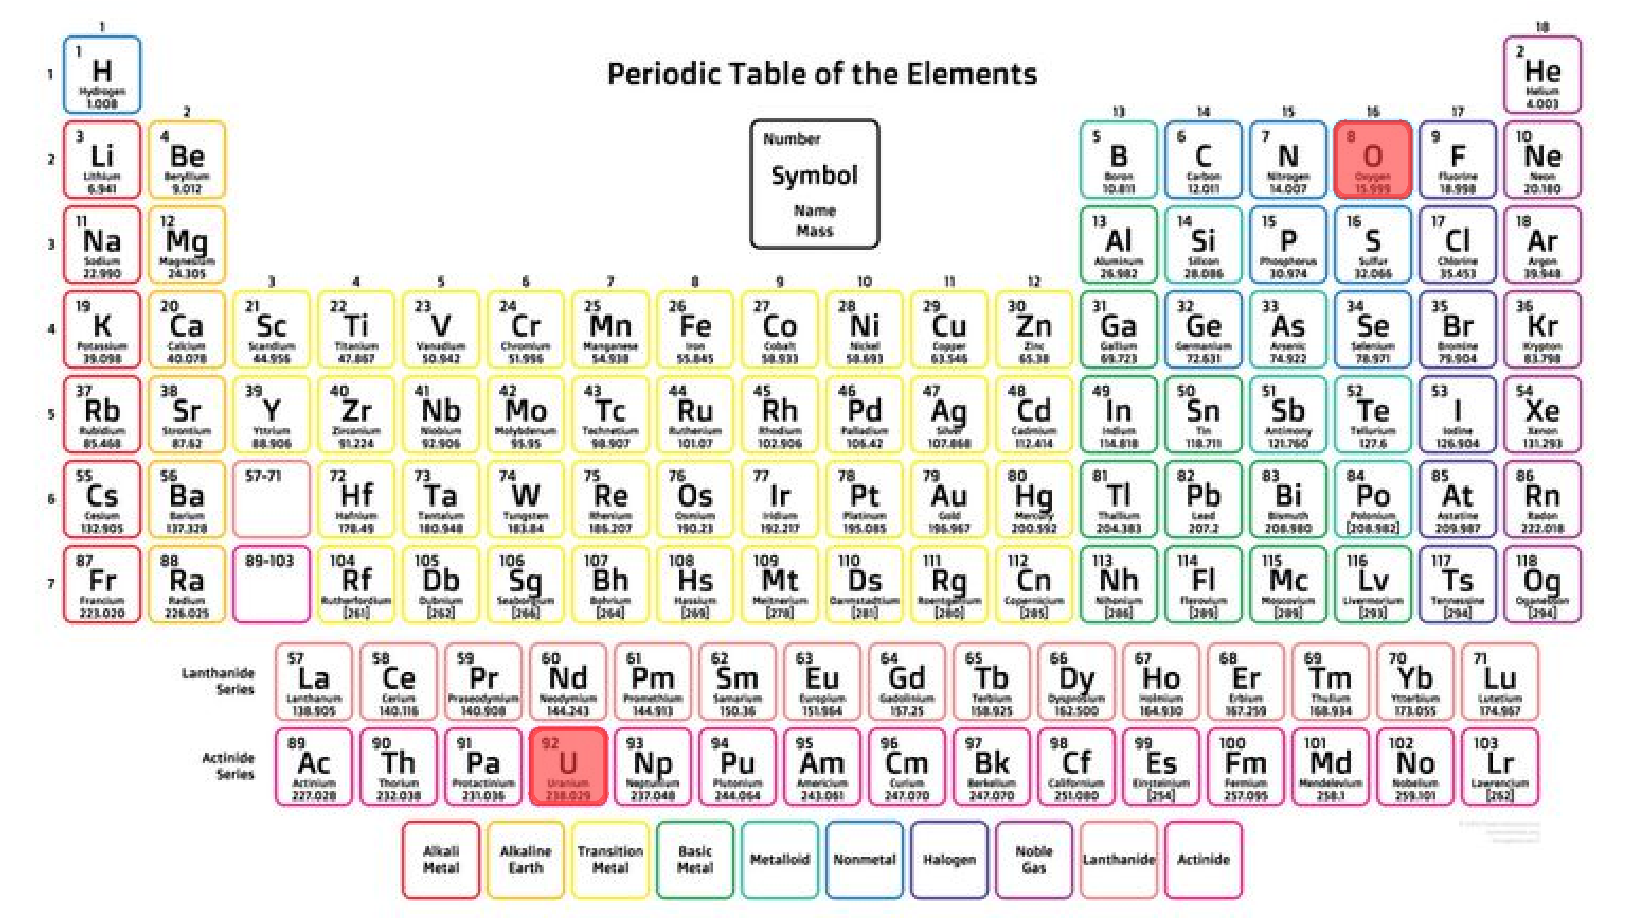
\includegraphics[width=\textwidth]{Figures/PT_BOL.pdf}
	\end{figure}
	}
	
	\only<3> {\begin{figure}
	\centering
	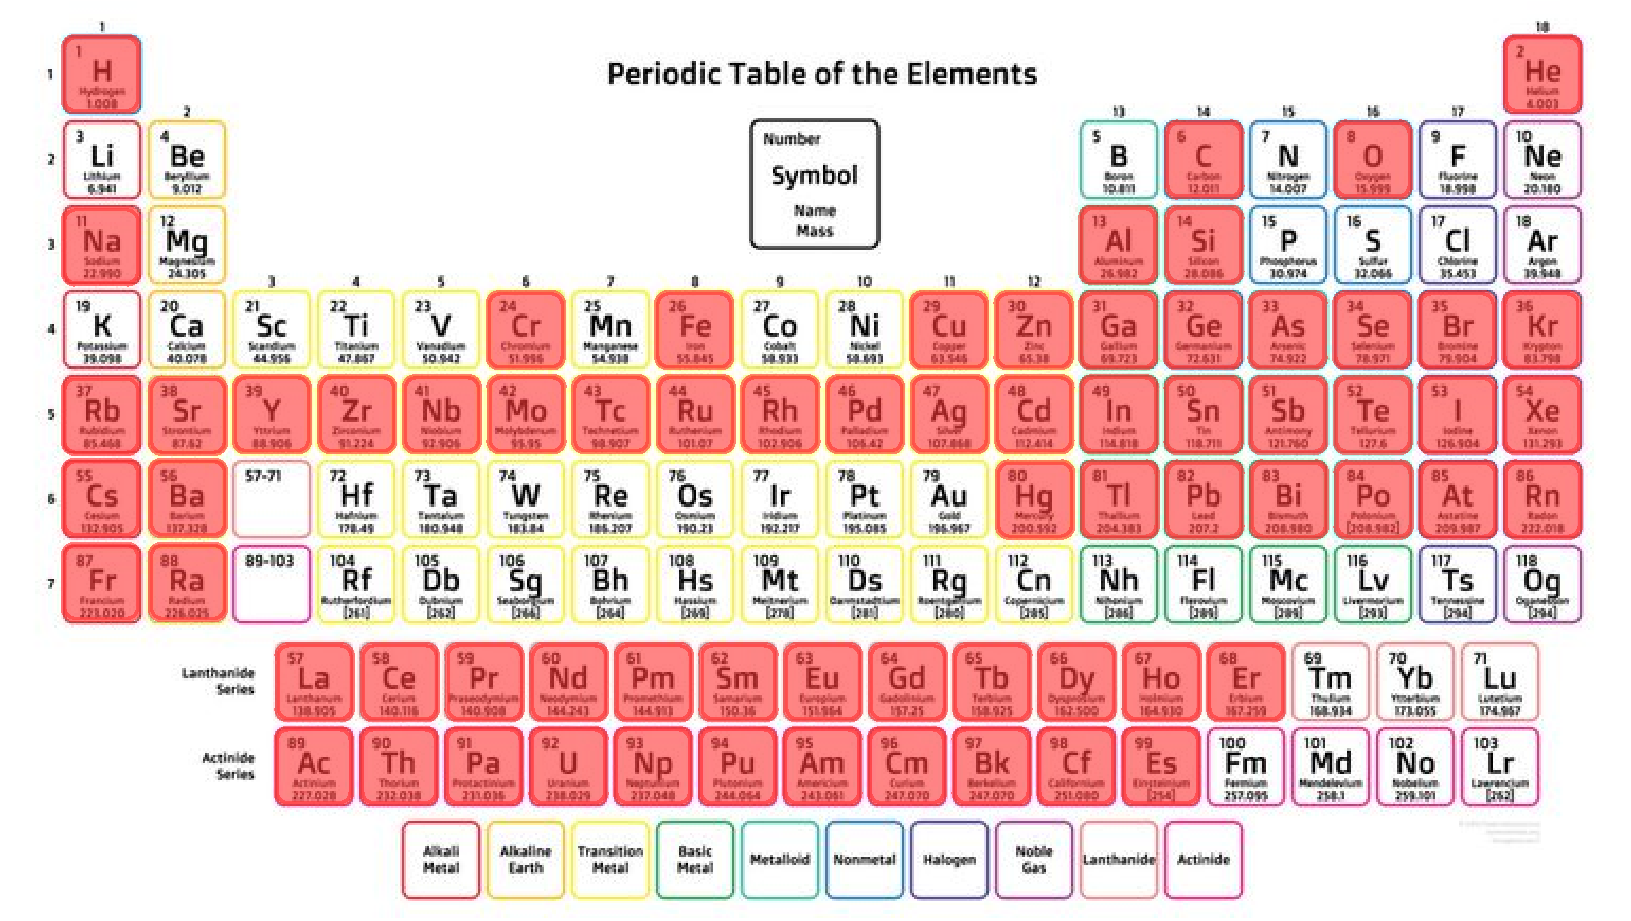
\includegraphics[width=\textwidth]{Figures/PT_EOL.pdf}
	\end{figure}
	}
}

\frame{
	\frametitle{Role of Thermochemistry}
	\onslide<1->{
		\begin{itemize}
			\item<1-> Experiments can not predict the material properties at every single point in the life of a nuclear material.
			\item<2-> Multiphysics simulations have to rely on empirical correlations of material properties.
			\item<3-> This reduces the accuracy of simulation.
			\item<4-> Thermochemistry allows us to capture the effect of compositional evolution on the properties of materials.
			\item<5-> Investigate phenomena which would be impossible to study using only experiments.
		\end{itemize}
	}
	
	\onslide<6->{\begin{figure}[htbp]
\begin{center}
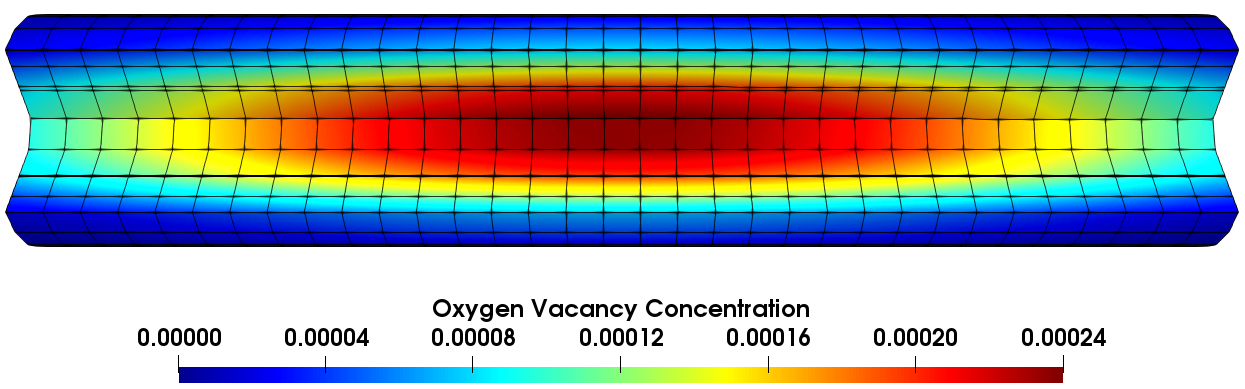
\includegraphics[width=\textwidth]{Figures/O_M}
\end{center}
\end{figure}
}
	}

\frame{
	\frametitle{Impetus}
	\begin{itemize}
		\item<+-> Direct coupling of thermochemical equilibrium calculations has only recently gained traction in the scientific community.
		\item<+-> Equilibrium calculations are extremely costly compared to other finite element based simulations.
		\item<+-> The material science community has traditionally relied on using phase diagrams and relatively simple material models in order to save computational cost.
		\item<+-> Most thermodynamic equilibrium softwares, such as ThermoCalc and FactSage, are commercial, standalone codes developed in 1990s.
		\item<+-> There is little freedom to make improvements or adapt them to specific needs.
		\item<+->	Thermochimica is an open-source code developed with the aim of direct coupling with multiphysics codes.
			\begin{itemize}
				\item Written in Fortran 90.
				\item Not developed within the MOOSE framework.
				\item Needs significant work to meet the NQA-1 standards.
			\end{itemize}
	\end{itemize}
}

\subsection{Outcomes}
\frame{
	\frametitle{Goals and Outcomes}
	\onslide<1->{\begin{block}{Goal of Research} \small
	The goal of this work is to develop a new state-of-the-art thermodynamic equilibrium code for direct integration in mutiphysics framework MOOSE.
	\end{block}}
	\onslide<2->{\begin{block}{Outcomes} \footnotesize
	\begin{enumerate}
		\item Development of a new advanced Gibbs energy minimiser written in C++ within the framework of MOOSE platform.
		\item Full integration within the multiphysics framework MOOSE, with the intent of coupling to the phase field code Marmot. 
		\item Enhanced initialisation algorithms to improve the computational performance.
		\item Investigation and implementation of robust global optimisation schemes to increase reliability and robustness.
		\item Software Quality Assurance  with rigorous verification and testing to comply with the NQA-1 guidelines required to be met for licensing.
	\end{enumerate}
	\end{block}}
}
%\section{Thermodynamic Equilibrium}
\subsection[Thermodynamic Potentials]{Gibbs energy and chemical potential}

\frame{
	\frametitle{Gibbs Energy}
	\begin{itemize}
	\item<1-> Developed  by Josiah Willard Gibbs in 1873.
%		\begin{block}{}
%		\textit{Available energy} is the greatest amount of mechanical work which can be obtained from a given quantity of a certain substance in a given initial state, without increasing its total volume or allowing heat to pass to or from external bodies, except such as at the close of the processes are left in their initial condition.
%		\end{block}
	\item<2-> Relates the \textit{enthalpy} of the system to its \textit{entropy}.
		\begin{exampleblock}{}
		\vspace{-0.25cm}
		\begin{equation*}
		G = H - TS
		\end{equation*}
		\end{exampleblock}
	\item<3-> Gibbs energy is the thermodynamic quantity that is minimised when a system reaches chemical equilibrium at constant temperature and pressure. 
	\end{itemize}
}

\frame{
	\frametitle{Chemical Potential}
	\begin{itemize}
		\item<1-> Chemical potential of species $i$ in phase $\lambda$ is a measure of the change in Gibbs energy of the system by the introduction of species $i$.
		\begin{exampleblock}{}
			\begin{equation*}
        				\mu_{i(\lambda)} = {\left (\frac{\partial G_{sys}}{\partial n_{i(\lambda)}} \right )}_{T,P,n_{j \neq i}}
    			\end{equation*}
		\end{exampleblock}
		
		\item<2-> Ideal mixing phases
		\begin{exampleblock}{}
		\vspace{-0.2cm}
			\begin{equation*}
        				\mu_{i(\lambda)} = g_{i(\lambda)}^0 + \ln x_{i(\lambda)}
    			\end{equation*}
		\end{exampleblock}
		
		\item<3-> Non-ideal mixing phases
		\begin{exampleblock}{}
		\vspace{-0.2cm}
			\begin{equation*}
        				\mu_{i(\lambda)} = g_{i(\lambda)}^0 + \ln x_{i(\lambda)} + g_{i(\lambda)}^{ex}
    			\end{equation*}
		\end{exampleblock}
	\end{itemize}	
}


\frame{
	\frametitle{Gibbs Energy}
	\begin{itemize}
	\item<1-> Integral Gibbs energy of a multicomponent, multiphase system can be expressed in terms of chemical potentials, $\mu_{i(\lambda)}$, of the species.
		\begin{block}{}
		\vspace{-0.15cm}
		\begin{equation*}
        			G_{sys} = RT \left ( \sum_{\lambda=1}^{\Lambda} n_{\lambda} \sum_{i=1}^{N_{\lambda}}x_{i({\lambda})}\tilde{\mu}_i + \sum_{\omega=1}^{\Omega} n_{\omega} \tilde{\mu}_{\omega} \right )
    		\end{equation*}
		\end{block}
	\item<2-> The Gibbs energy of  the system can also be expressed in terms of the element potentials, $\Gamma_j$, and the number of moles, $b_j$, of the system components.
		\begin{exampleblock}{}
		\vspace{-0.15cm}
		\begin{equation*}
		G_{sys} = \sum_{j=1}^{C} \Gamma_j b_j
		\end{equation*}
		\end{exampleblock}
	\end{itemize}
}

\subsection{Conditions of Thermodynamic Equilibrium}
\frame{
	\frametitle{Thermodynamic Equilibrium - Necessary Conditions}
	\pause
	\begin{block}{Conservation of mass}
		\begin{equation*}
		b_j = \sum_{\lambda=1}^{\Lambda} n_{\lambda}\sum_{i=1}^{N_{\lambda}}x_{i({\lambda})}{\nu}_{i,j} +  \sum_{\omega=1}^{\Omega} n_{\omega}{\nu}
		\end{equation*}
	\end{block}
	\pause
	\begin{exampleblock}{Gibbs' phase rule}
		\vspace{-0.1cm}
		\begin{equation*}
		F=C-\Phi + 2 + \Xi
		\end{equation*}
	\end{exampleblock}
	\pause
	\begin{alertblock}{Gibbs' Criteria}
		\begin{equation*}
		\mu_{i} = \sum_{j=1}^C \nu_{i,j} \Gamma_j
		\end{equation*}
	\end{alertblock}		
}

\frame{
	\frametitle{Thermodynamic Equilibrium - Sufficient Conditions}
	\only<1-2>{\onslide<1-2>{
	\begin{block}{Gibbs plane}
	\begin{equation*}
		\pi_{\lambda} = \min_{\lambda} \sum_{i=1}^{N_{\lambda}}x_{i({\lambda})} \left (\mu_{i({\lambda})} - \sum_{j=1}^C \nu_{i,j}\Gamma_j \right )
	\end{equation*}
	\end{block}}
	
	\onslide<2>{
	\begin{block}{Constraints}
	\vspace{-0.25cm}
	\begin{align*}
		\sum_{i=1}^{N_{\lambda}} x_{i(\lambda)} = 1 \\
		x_{i(\lambda)}} \geq 0 %\mspace{50mu} \forall i
	\end{align*}
	\end{block}}
	
	\only<3>{
	\begin{figure}[htbp]
		\begin{center}
		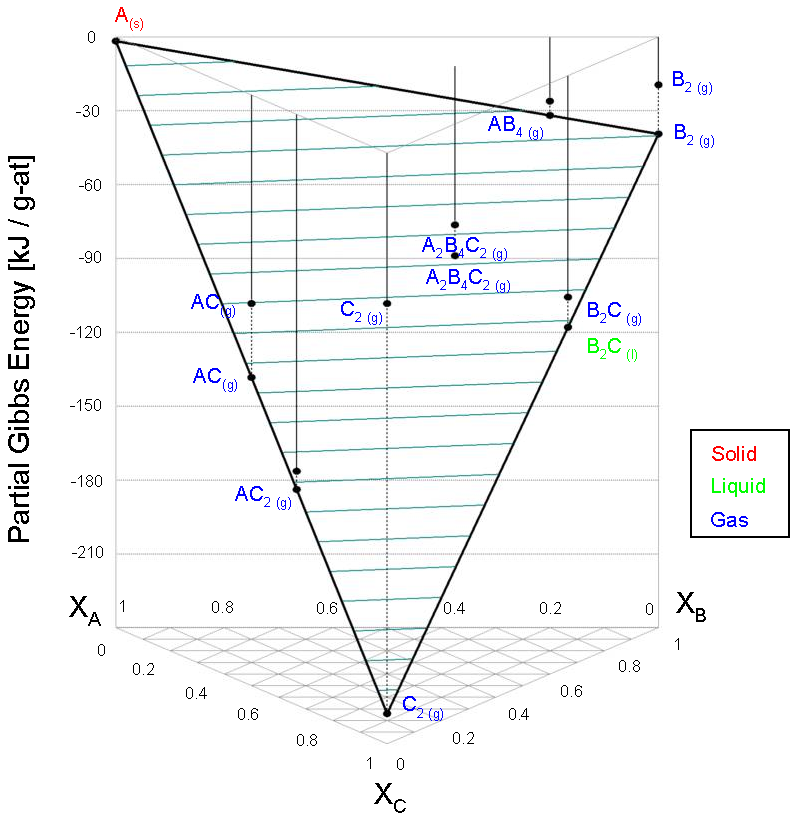
\includegraphics[height=0.75\paperheight]{Figures/Gibbs_plane}
		\end{center}
	\end{figure}
	}
}

\subsection{Gibbs Energy Minimisation}
\frame{
	\frametitle{Gibbs Energy Minimisation}
	\only<1-3>{\begin{itemize}
		\item<1-> Gibbs Energy Minimisation was proposed in 1958 by White, Jonson and Dantzig and is used almost ubiquitously in computation of thermodynamic equilibrium.
		\item<2-> Second order steepest descent method.
		\item<3-> Constrains Gibbs' phase rule while simultaneously minimising the mass balance and Gibbs' criteria residuals.
	\end{itemize}}
	\only<4>{\begin{alertblock}{Optimise}
		\begin{equation*}
		b_j = \sum_{\lambda=1}^{\Lambda} n_{\lambda}\sum_{i=1}^{N_{\lambda}}x_{i({\lambda})}{\nu}_{i,j} +  \sum_{\omega=1}^{\Omega} n_{\omega}{\nu}
		\end{equation*}
	\end{alertblock}
	\begin{exampleblock}{Constraint}
		\vspace{-0.1cm}
		\begin{equation*}
		F=C-\Phi + 2 + \Xi
		\end{equation*}
	\end{exampleblock}
	\pause
	\begin{alertblock}{Optimise}
		\begin{equation*}
		\mu_{i} = \sum_{j=1}^C \nu_{i,j} \Gamma_j
		\end{equation*}
	\end{alertblock}	}
}

%\section{Computational Implementation}
\subsection[Overview]{Gibbs Energy Minimiser - Overview}

\frame{
	\frametitle{Computational Structure}
	\begin{figure}[htbp]
		\begin{center}
		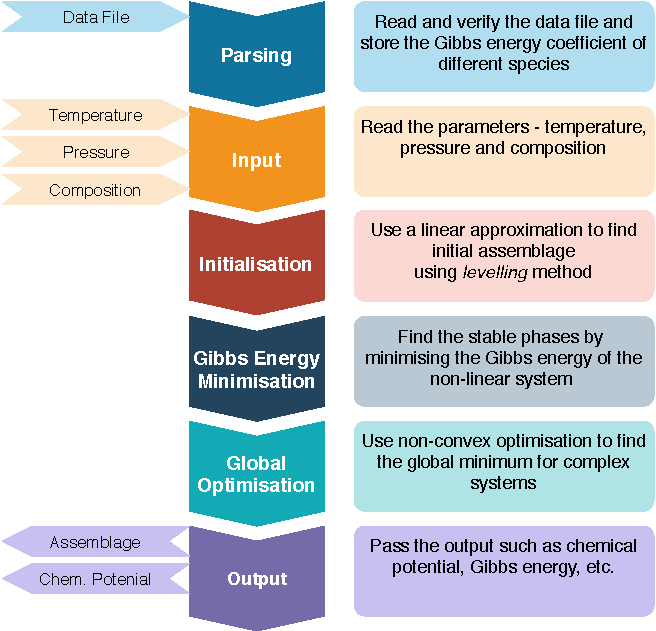
\includegraphics[height=0.65\paperheight]{Figures/YJ_structure.pdf}
		\end{center}
	\end{figure}
}

\subsection{Gibbs Energy Minimiser}
    \frame{
    \frametitle{Parsing and Input}
    
         \only<1>{
             \begin{itemize}
                 \item<1-> The data files are created using the Calphad method and are available in different formats.
             \end{itemize}
             }
         \only<2>{\begin{figure}
                 \centering
                 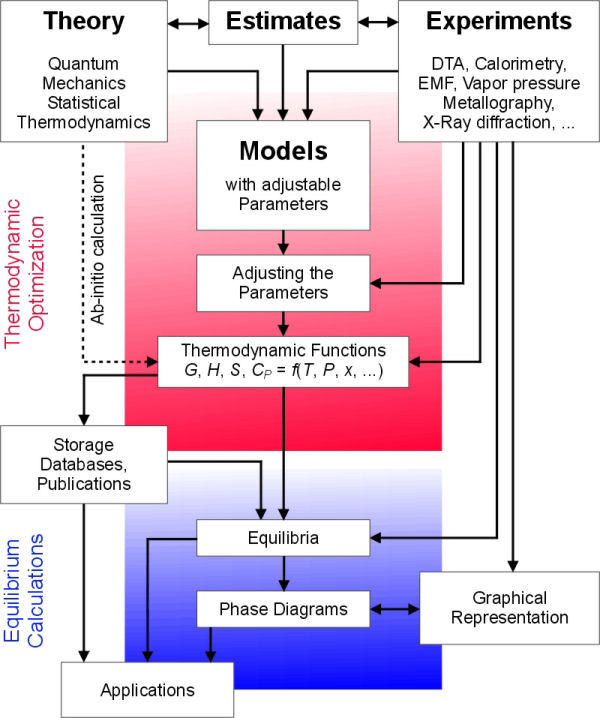
\includegraphics[height=0.75\paperheight]{Figures/Calphad_method.jpg}
             \end{figure}}
         \only<3>{
             \begin{itemize}
                 \item<3-> The data files are created using the well known Calphad method and can be available in different formats.
                 \item<3-> Most commonly used formats are ThermoCalc (*.tdb) and FactSage (*.dat).
                 \item<3-> Yellowjacket uses ChemSage (*.dat) format datafiles, which can be generated by the commercial software FactSage.
                 \item<3-> Temperature, pressure and composition are required at each time step and for each mesh element.
                 \item<3-> At each time step MOOSE can provide these inputs to Yellowjacket.
             \end{itemize}}
  }

    \frame{
    \frametitle{Initialisation}
             \begin{itemize}
                 \item Gibbs energy minimisers require an initial estimate of molar quantities of species and phases.
                 \item \textit{Levelling} is an estimating process developed by Eriksson and Thompson (1989).
                 \item Levelling temporarily converts the non-linear optimisation problem into a linear optimisation problem by treating all species and phases as pure separate phases.
                 \item The number of iterations required to achieve convergence does not increase rapidly with the number of system components.
             \end{itemize}
    }
    
%      \frame{
%    \frametitle{Initialisation}
%         \begin{figure}
%             \centering
%             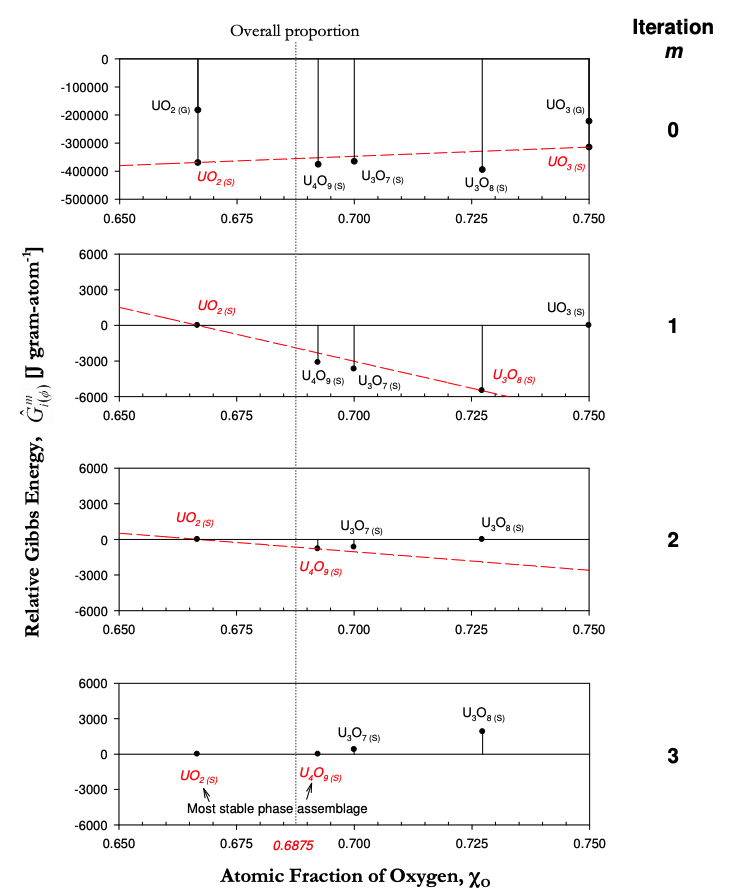
\includegraphics[height=0.75\paperheight]{Figures/Levelling_illustration}
%         \end{figure}
%      }
    
%    \frame{
%    \frametitle{Initialisation}
%     \begin{multicols}{2}
%         \begin{itemize}
%             \item Initialise using neighbour cells
%             \begin{figure}
%                 \centering
%                 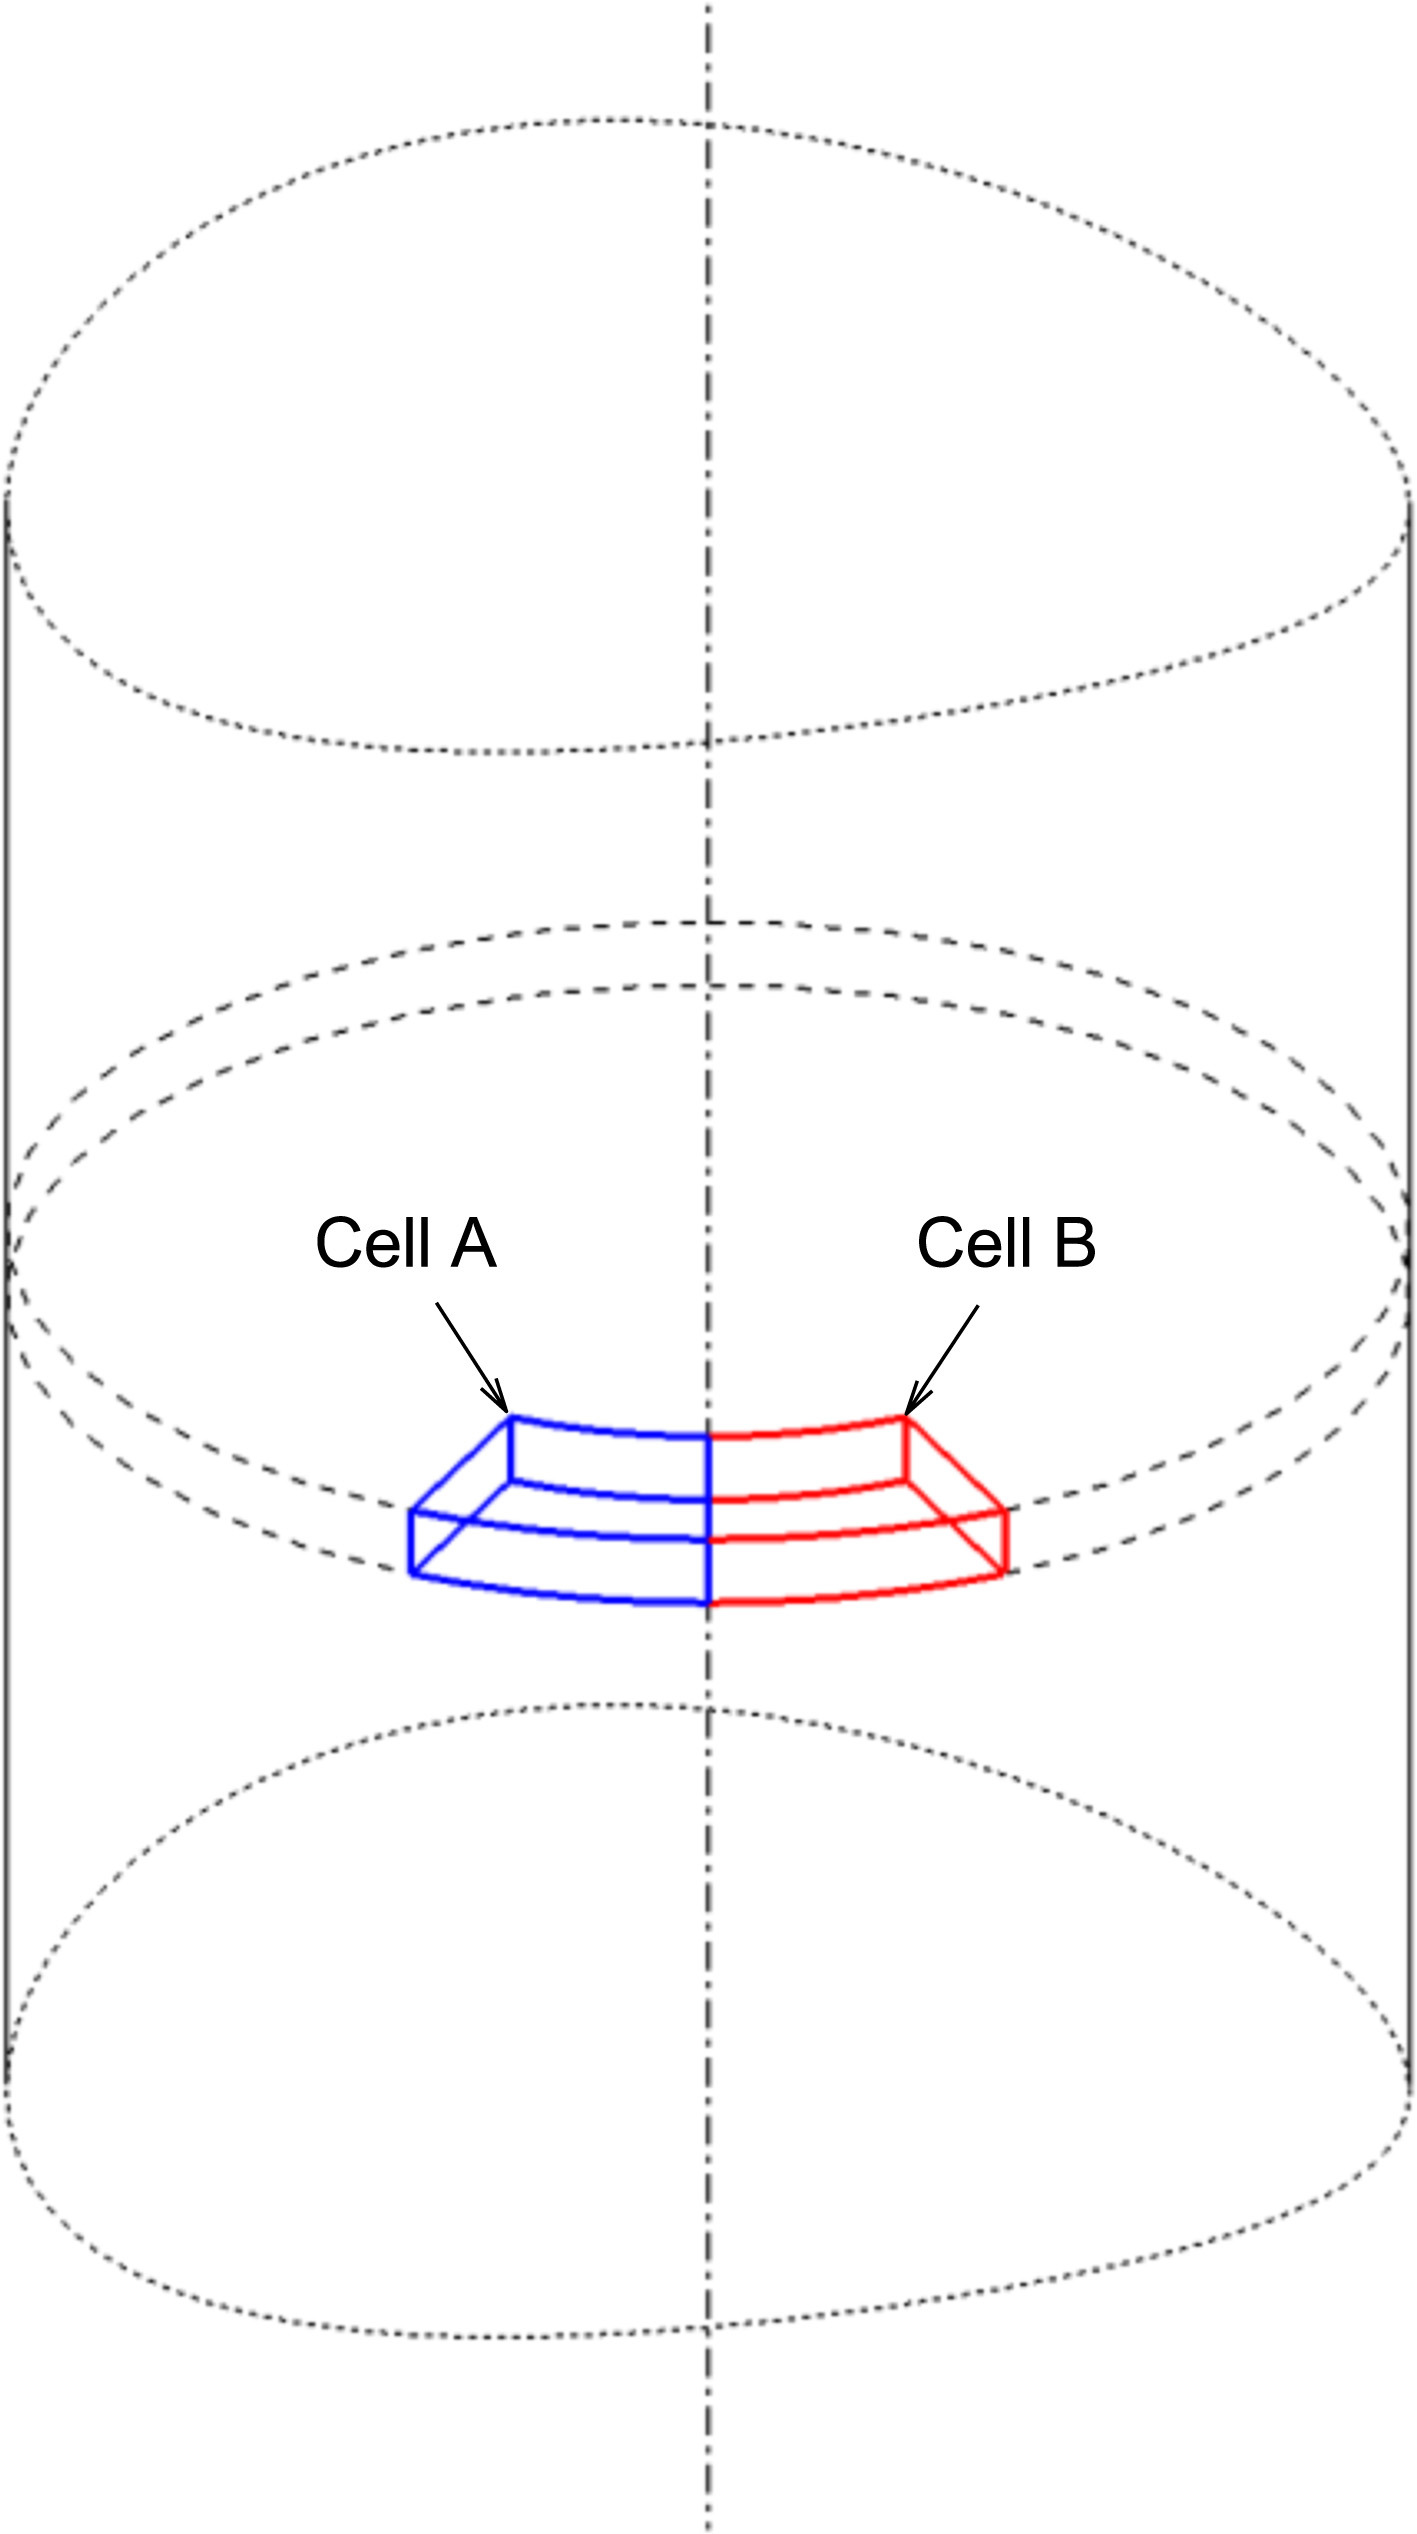
\includegraphics[width=0.575\linewidth]{Figures/rest.jpg}
%             \end{figure}
%         \end{itemize}
%         \columnbreak
%         \begin{itemize}
%             \item Initialise with last time step
%             \begin{figure}
%                 \centering
%                 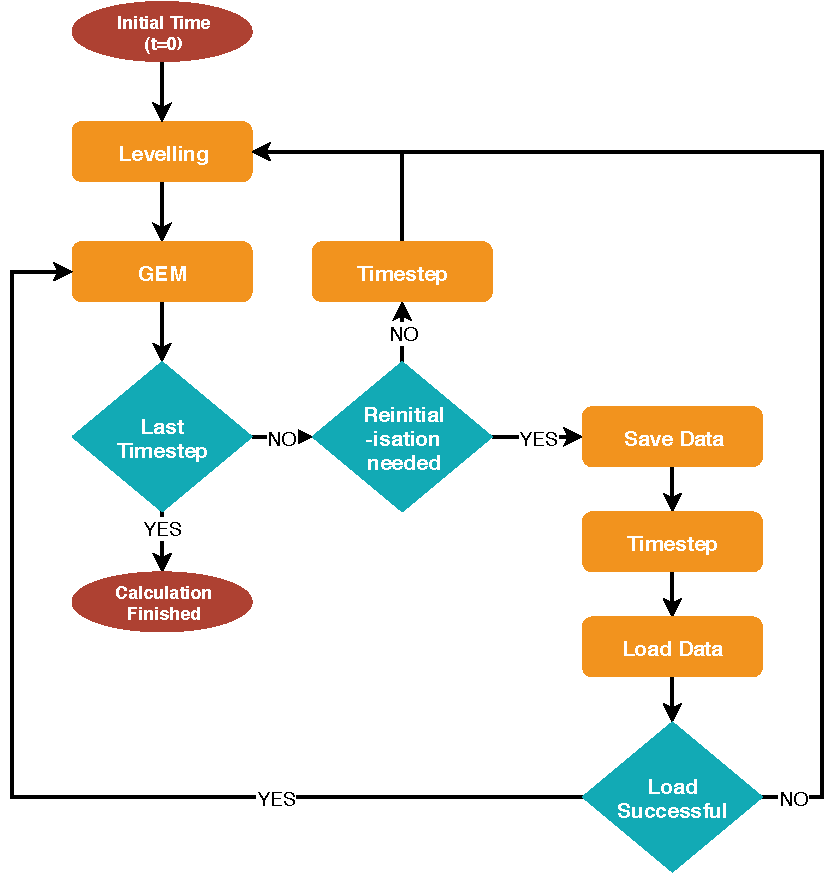
\includegraphics[width=0.925\linewidth]{Figures/Initialisation.pdf}
%             \end{figure}
%         \end{itemize}
%     \end{multicols}
%    }

    
     \frame{
     \frametitle{Gibbs Energy Minimisation}
         \onslide<1-4>{\begin{itemize}
 	        \item<1-> GEM uses the method of Lagrange multipliers resulting in the following system of equations \[\mtx{H}\cdot\vec{\pi}=\vec{\zeta}\]
 	    \end{itemize}}
	    \scriptsize
\only<2>{\begin{equation*}\label{eq:Hessian_mat}
        \mathbf{H} = 
        \begin{bmatrix}
            r_{j=1,k=1} & \dots & r_{j=1,k=C} & \phi_{j=1,\lambda=1} & \dots & \phi_{j=1,\lambda=\Lambda} & \nu_{j=1,\omega=1} & \dots & \nu_{j=1,\omega=\Omega} \\
            \vdots & \ddots & \vdots & \vdots & \ddots & \vdots & \vdots & \ddots & \vdots \\
            r_{j=C,k=1} & \dots & r_{j=C,k=C} & \phi_{j=C,\lambda=1} & \dots & \phi_{j=C,\lambda=\Lambda} & \nu_{j=C,\omega=1} & \dots & \nu_{j=C,\omega=\Omega} \\
            \phi_{\lambda=1,j=1} & \dots & \phi_{\lambda=1,j=C} & 0 & \dots & 0 & 0 & \dots & 0 \\
            \vdots & \ddots & \vdots & \vdots & \ddots & \vdots & \vdots & \ddots & \vdots \\
            \phi_{\lambda=\Lambda,j=1} & \dots & \phi_{\lambda=\Lambda,j=C} & 0 & \dots & 0 & 0 & \dots & 0 \\
            \nu_{\omega=1,j=1} & \dots & \nu_{\omega=1,j=C} & 0 & \dots & 0 & 0 & \dots & 0 \\
            \vdots & \ddots & \vdots & \vdots & \ddots & \vdots & \vdots & \ddots & \vdots \\
            \nu_{\omega=\Omega,j=1} & \dots & \nu_{\omega=\Omega,j=C} & 0 & \dots & 0 & 0 & \dots & 0 
        \end{bmatrix}
         \end{equation*}
         $$
        	r_{j,k} = \sum_{\lambda=1}^{\Lambda} \sum_{i=1}^{N_\lambda} n_{i(\lambda)} \nu_{i,j}\nu_{i,k} \mspace{25mu} \phi_{\lambda,j} = \sum_{i=1}^{N_\lambda} n_{i(\lambda)} \nu_{i,j}
        $$
         }
    
    \only<3>{ \begin{equation*}\label{eq:LagMult_mat}
        \boldsymbol{\pi} = 
        \begin{bmatrix}
            \pi_{j=1}^{m+1} \\
            \vdots \\
            \pi_{j=E}^{m+1} \\
            \pi_{\lambda=1}^{m+1} \\
            \vdots \\
            \pi_{\lambda=\Lambda}^{m+1} \\
            \pi_{\omega=1}^{m+1} \\
            \vdots\\
            \pi_{\omega=\Omega}^{m+1}
        \end{bmatrix}
    \end{equation*}}
    
    \only<4>{ \begin{equation*}\label{eq:Constraint_mat}
        \boldsymbol{\zeta} = 
        \begin{bmatrix}
            b_{j=1} +  \sum_{\lambda=1}^{\Lambda} \sum_{i=1}^{N_\lambda} \left( \frac{\mu_{i(\lambda)}^{m}}{RT} -1 \right)n_{i(\lambda)}^{m} \nu_{i,j=1}\\
            \vdots \\
            b_{j=E} +  \sum_{\lambda=1}^{\Lambda} \sum_{i=1}^{N_\lambda} \left( \frac{\mu_{i(\lambda)}^{m}}{RT} -1 \right)n_{i(\lambda)}^{m} \nu_{i,j=E}\\
            \sum_{i=1}^{N_{\lambda=1}} \left( \frac{\mu_{i(\lambda=1)}^{m}}{RT} -1 \right)n_{i(\lambda=1)}^{m} \\
            \vdots \\
            \sum_{i=1}^{N_{\lambda=\Lambda}} \left( \frac{\mu_{i(\lambda=\Lambda)}^{m}}{RT} -1 \right)n_{i(\lambda=\Lambda)}^{m} \\
            \frac{\mu_{\omega=1}^{m}}{RT} \\
            \vdots\\
            \frac{\mu_{\omega=\Omega}^{m}}{RT} \\
        \end{bmatrix}
    \end{equation*}
}
    }
    
%     \begin{frame}{Gibbs Energy Minimisation}
%         \begin{itemize}
% 	        \item Phase assemblage algorithm
% 	    \end{itemize}
% 	    \begin{figure}
% 	        \centering
% 	        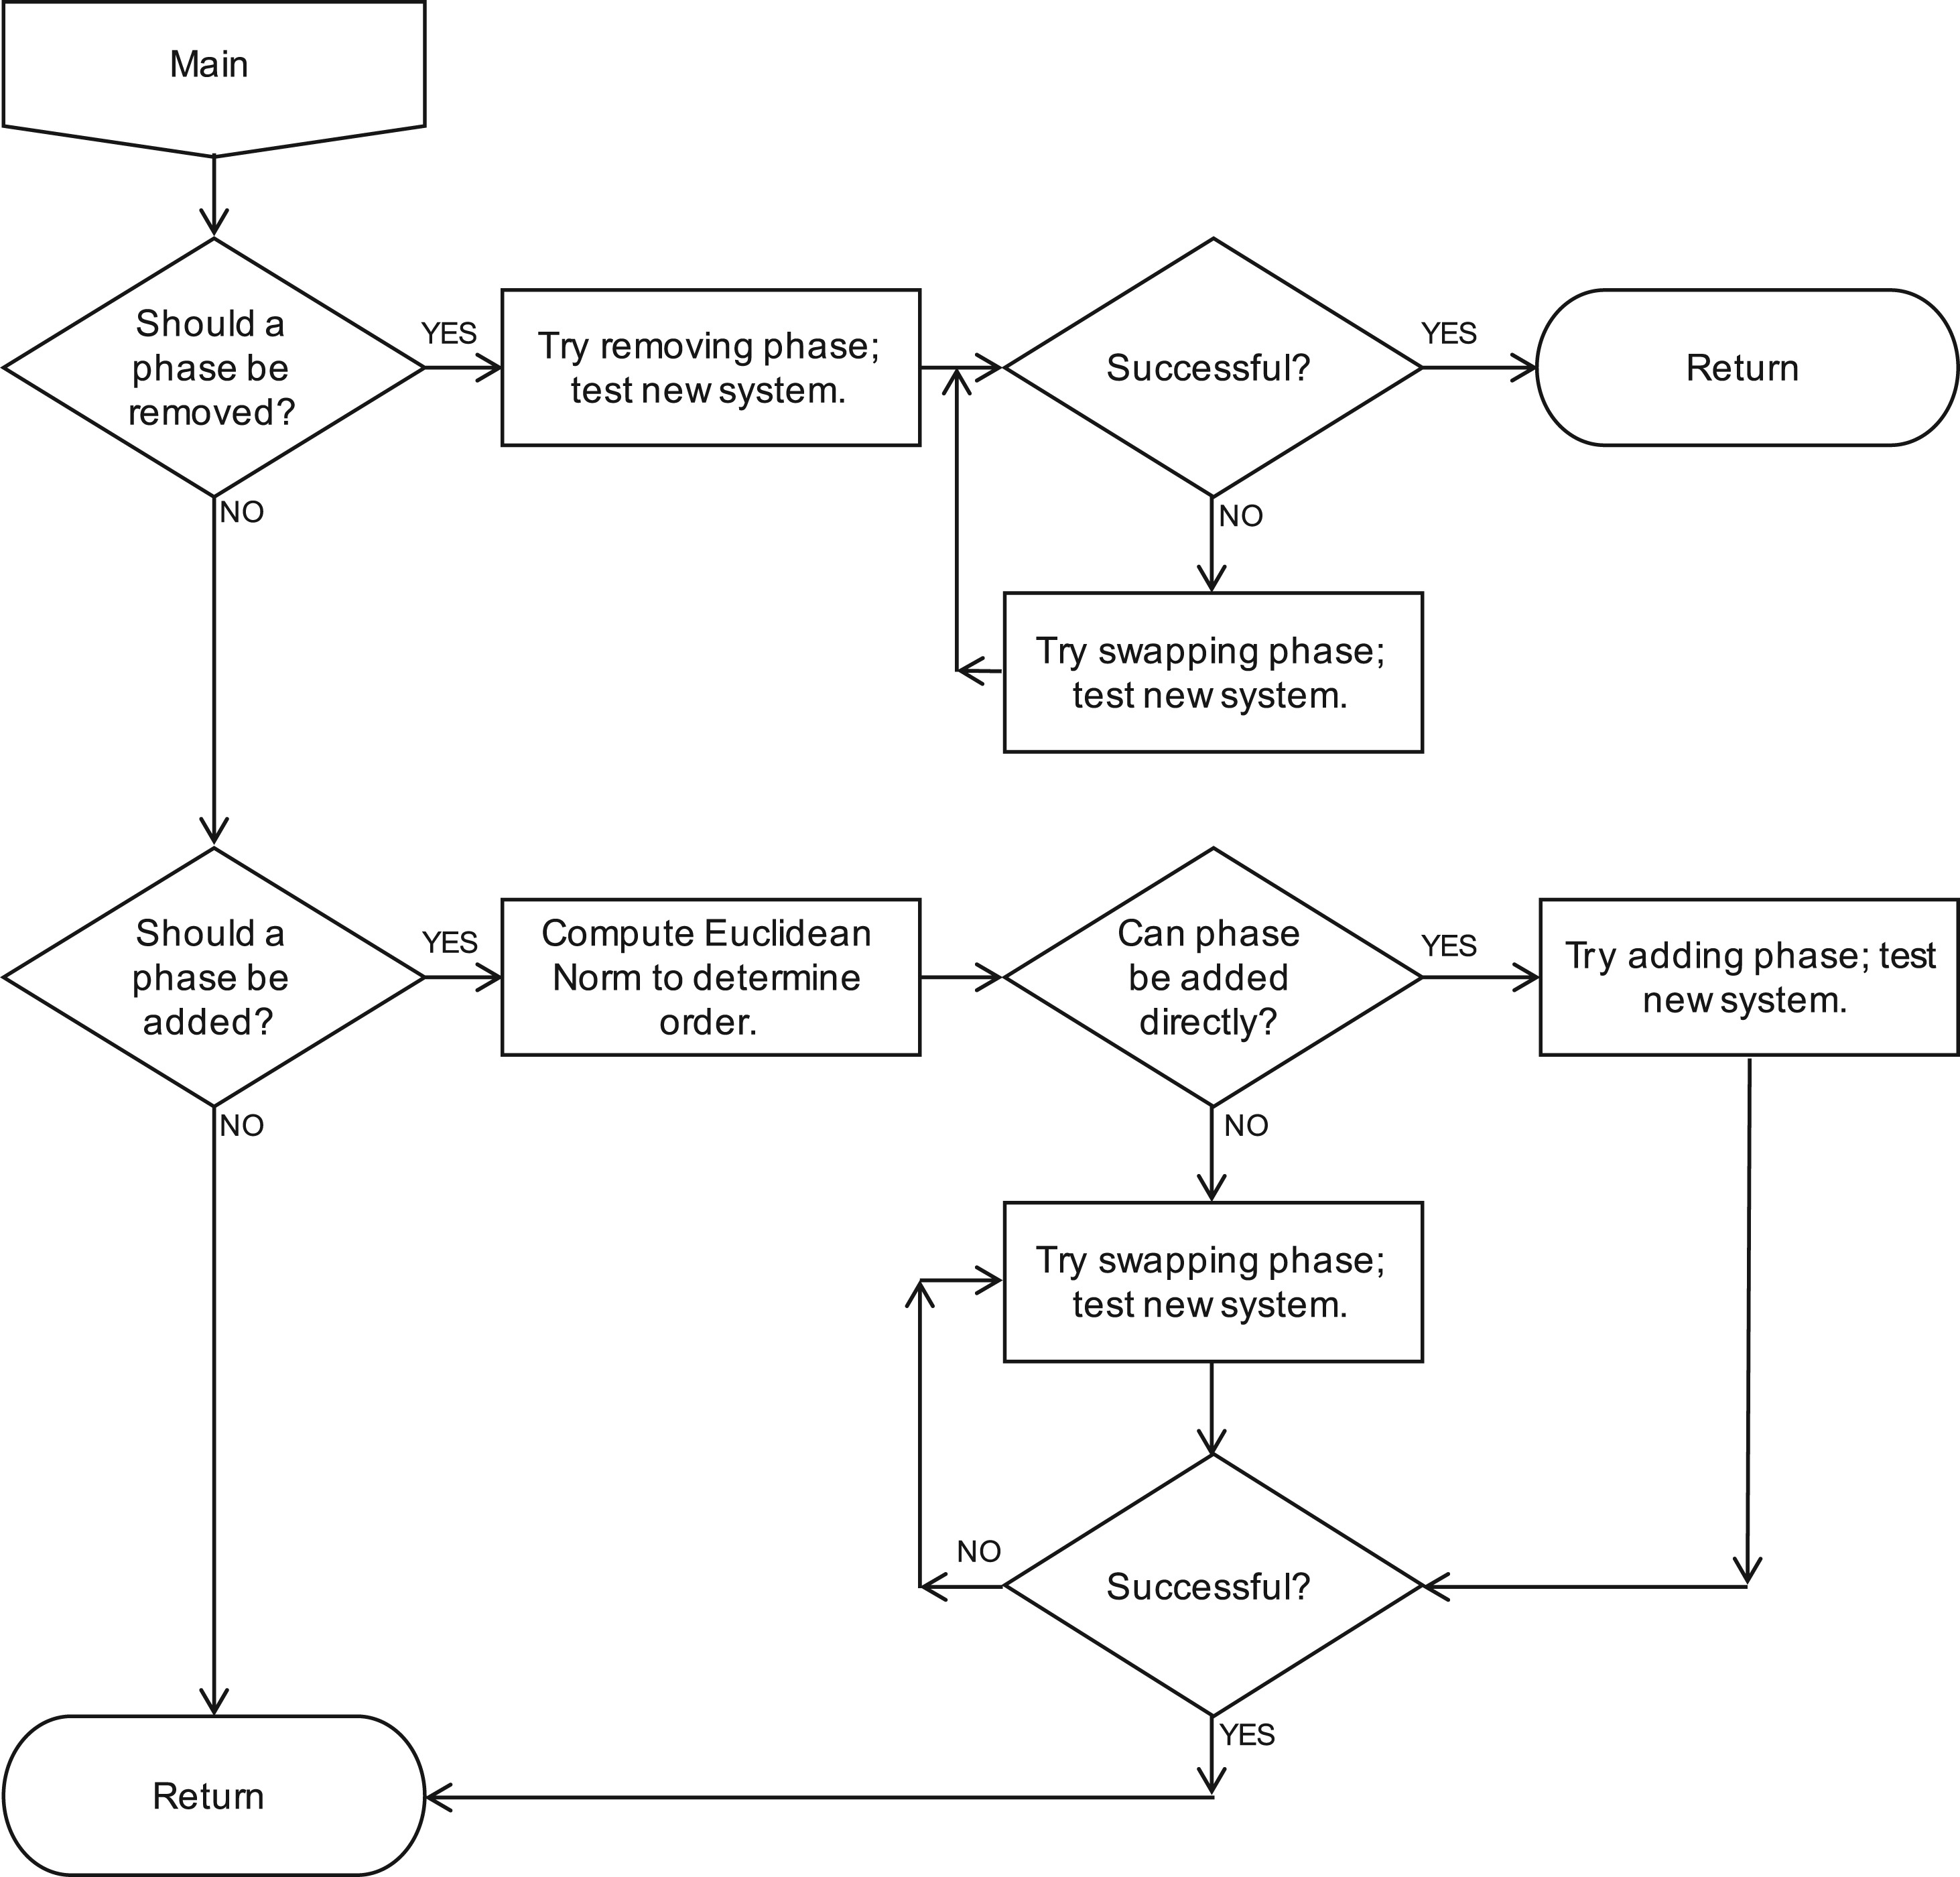
\includegraphics[width=0.45\linewidth]{Figures/Phase_assemblage.jpg}
% 	    \end{figure}
%     \end{frame}
%    
%     \begin{frame}{Gibbs Energy Minimisation}
%         \begin{itemize}
% 	        \item Line Search algorithms
% 	   % \end{itemize}
% 	    \begin{figure}
% 	        \centering
% 	        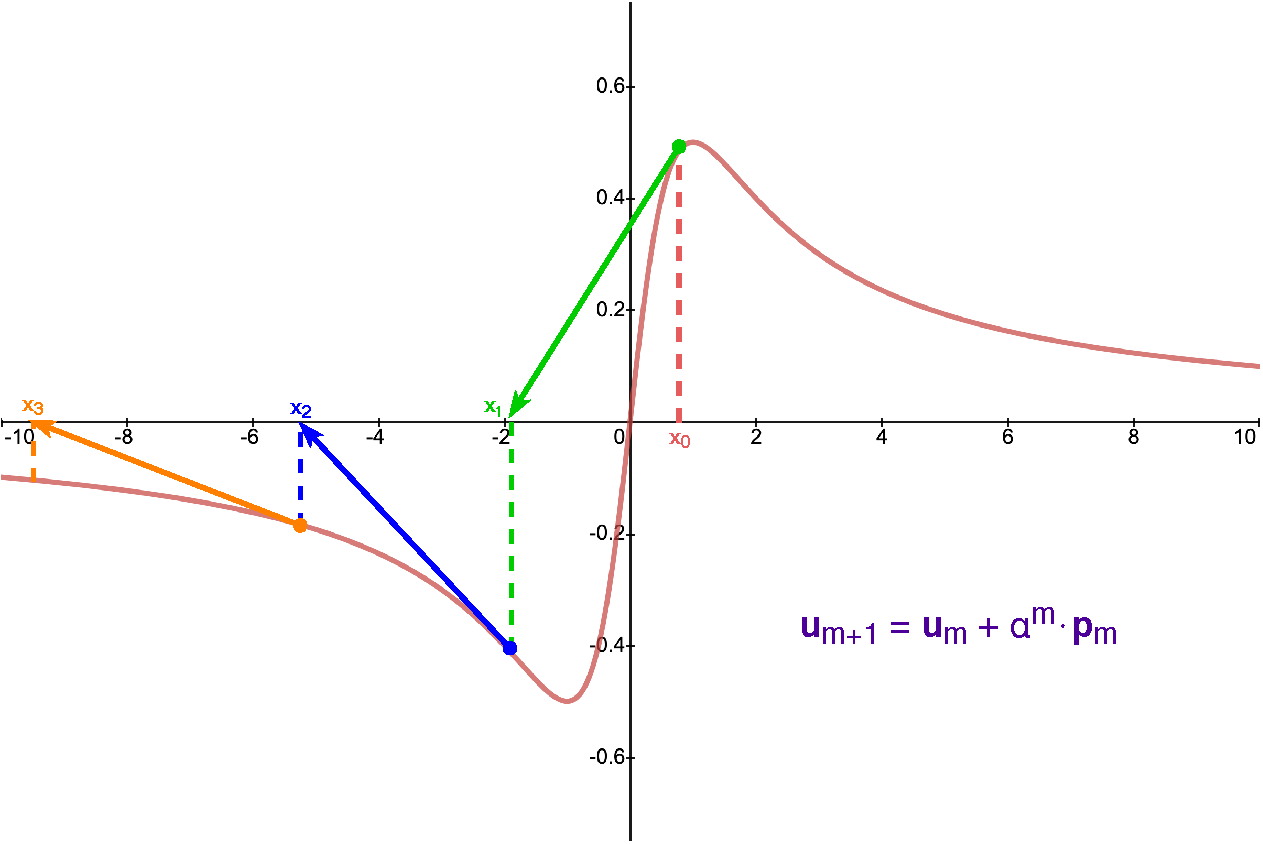
\includegraphics[width=0.5\paperwidth]{Figures/Line_search.pdf}
% 	    \end{figure}
% 	   % \begin{itemize}
% 	        \item Use of Wolfe/Armijo conditions can help avoid divergence.
% 	    \end{itemize}
%     \end{frame}
    
     \begin{frame}{Global Optimisation}
         \begin{itemize}
             \item The Gibbs energy function of non-ideal phases may be non-convex, yielding multiple local minima. This makes finding global minimum a challenge.
         \end{itemize}
         \begin{figure}
             \centering
             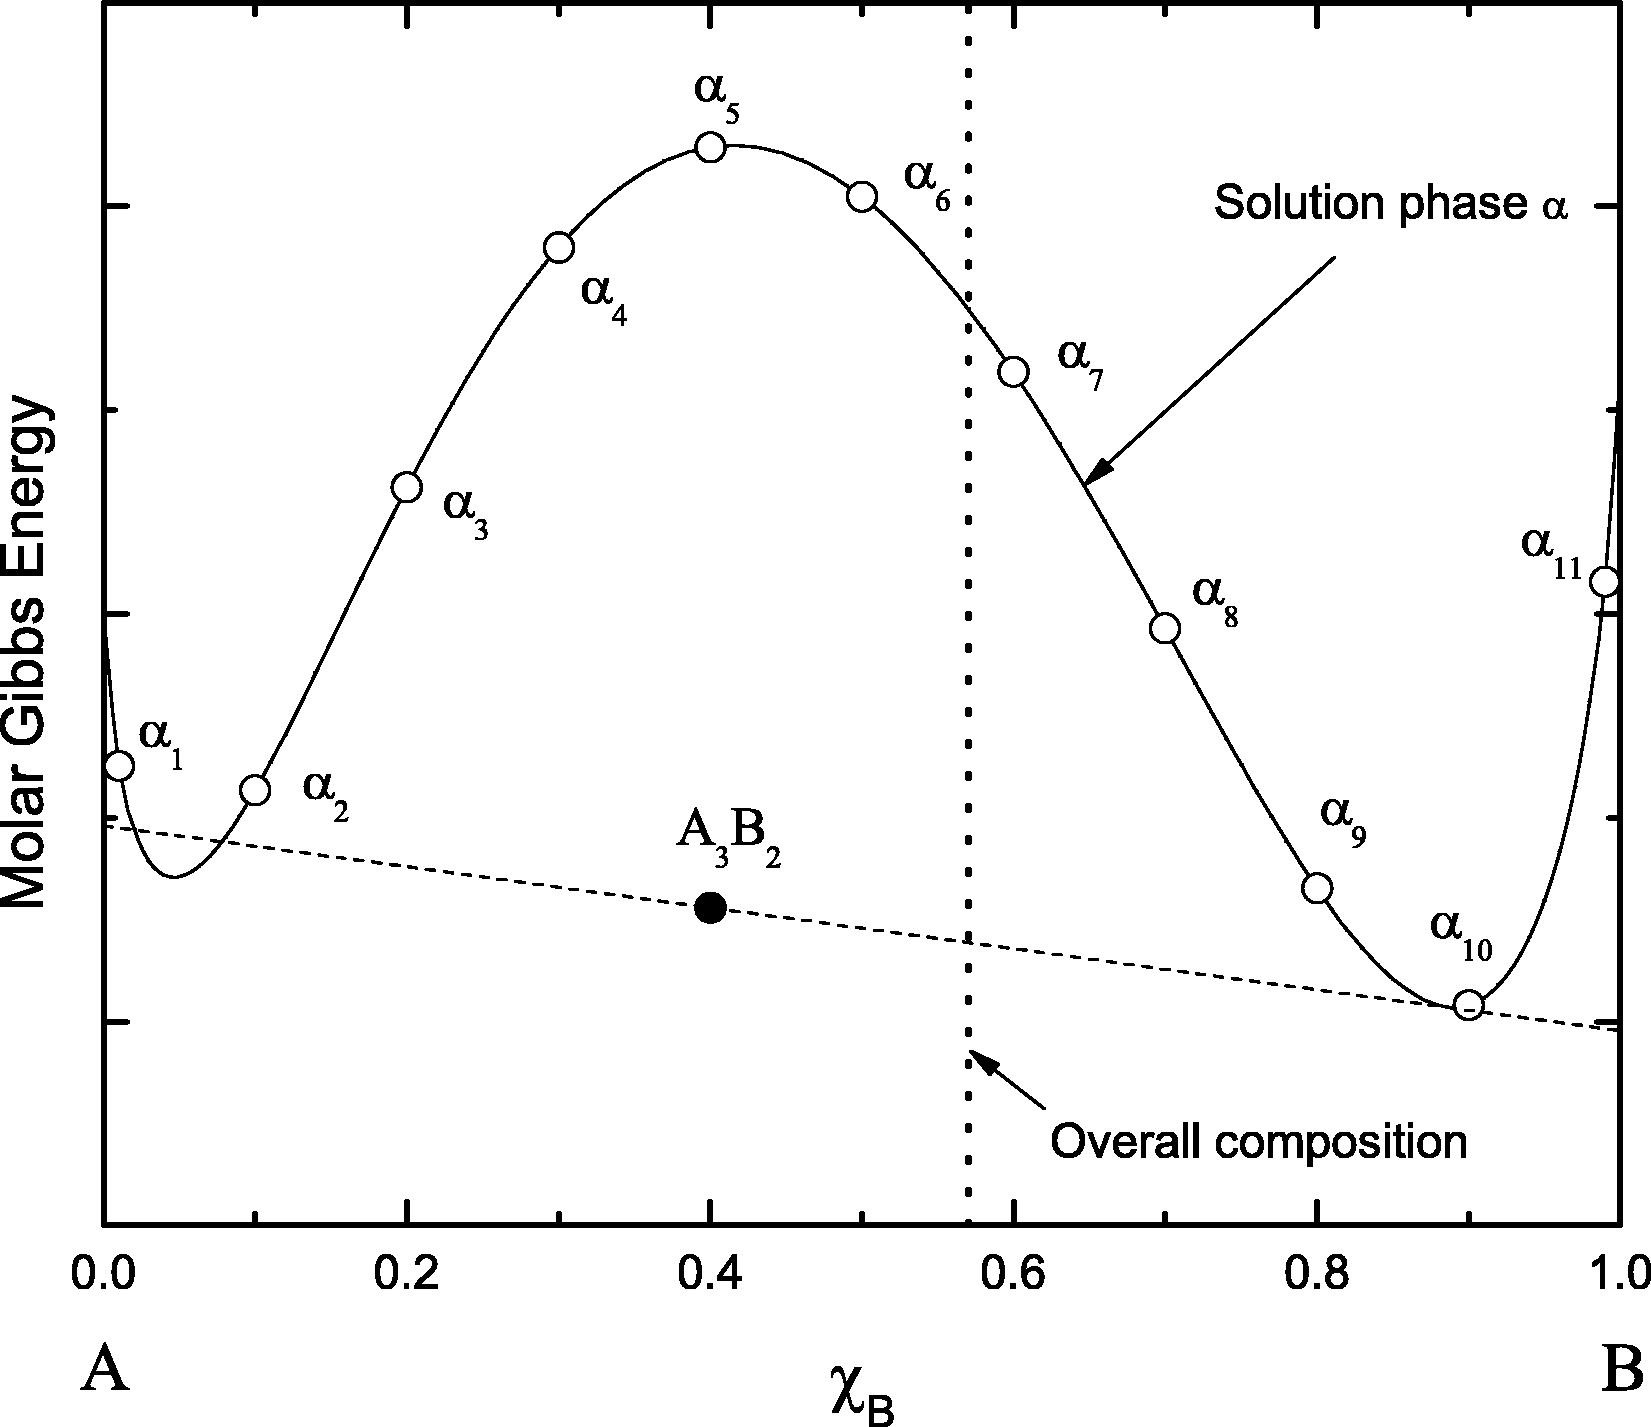
\includegraphics[width=0.5\linewidth]{Figures/Global_opt1}
         \end{figure}
         \blfootnote{Image - Piro \& Simunovic, Comput. Mater. Sci, 118, 87-96, 2016. }
     \end{frame}
    

     \begin{frame}{Output}
         \begin{itemize}
             \item Outputs after the Gibbs energy minimisation and global optimisation include moles of phases, species mole fraction in each phase, chemical potentials, Gibbs energy, etc.
             \item The chemical potential of various species can be used to find the driving force for other reactions such as corrosion.
             \item These parameters can also be passed to other MOOSE based codes such as {Marmot} and {Bison}.
         \end{itemize}
     \end{frame}
     
     \subsection{Challenges and Thrust Areas}
     \frame{
     	\frametitle{Challenges and Thrust Areas}
	\begin{itemize}
		\item<1-> Initialisation
			\begin{itemize}
				\item<1-> Levelling + GEM can often be costly in multiphysics simulations.
				\item<1-> Principles of continuum can be used to reduce the computational time.
				\item<1-> Using solution from previous time step as initial estimate. For example,  Thermochimica - Bison coupled problems have been accelerated by up to 7X.
				\item<1-> Assemblage from a neighbouring element can potentially be used as an initialisation method.	
			\end{itemize}
		\item<2-> Gibbs Energy Minimisation
			\begin{itemize}
				\item<2-> There is a need to constantly update the phases present in the assemblage - phases might have to be removed, added or exchanged.
				\item<2-> Phase selection algorithm can eliminate cycling.
				\item<2-> Line search methods can significantly affect the rate of convergence of Newton solver.
				\item<2-> Armijo/Wolfe conditions must be efficiently implemented to make sure that Newton steps do not lead to divergence.
			\end{itemize}
	\end{itemize}
     }
     
     \frame{
     	\frametitle{Challenges and Thrust Areas}
	\only<1>{
	\begin{itemize}
		\item<1-> Global Optimisation
			\begin{itemize}
				\item<1-> Mathematically, global optimisation implies finding the Gibbs plane that satisfies the sufficient condition: \[\pi_{\lambda} = \min_{\lambda} \sum_{i=1}^{N_{\lambda}}x_{i({\lambda})} \left (\mu_{i({\lambda})} - \sum_{j=1}^C \nu_{i,j}\Gamma_j \right )\]
            			\item<1-> No global optimisation technique guarantees the ability of finding a global extremum of a non-convex function.
             			\item<1-> Searching for a global minimum becomes increasingly more difficult as the size of the system increases.
             			\item<1-> The computational effort associated with performing this task can increase very rapidly in large systems.
			\end{itemize}
	\end{itemize}}
	\only<2>{
			\begin{itemize}
				\item<2-> Most commercial codes do not specify the global optimisation method used.
				\item<2-> Originally, they relied on the grid construction method which is a brute force method.
				\begin{figure}
            				\centering
            				 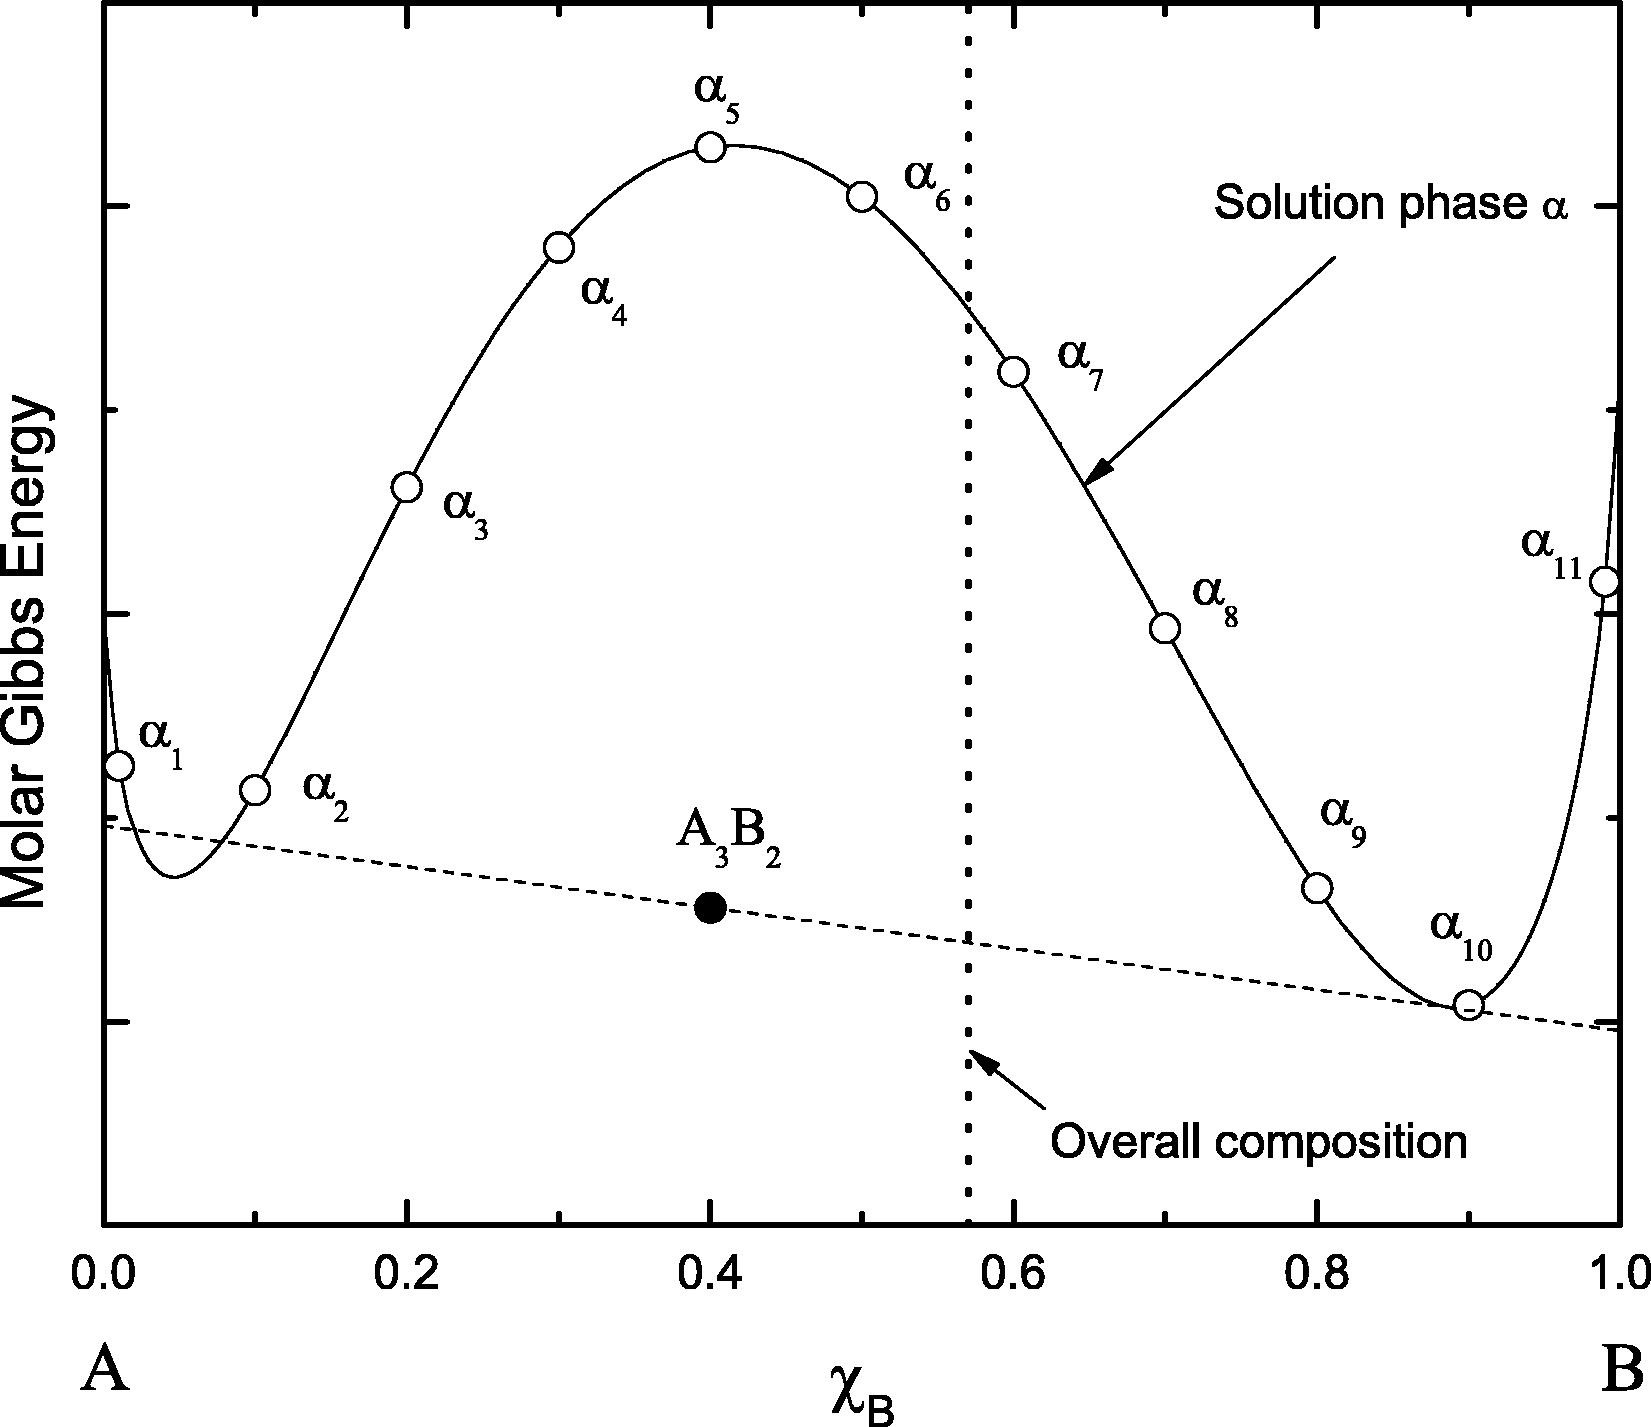
\includegraphics[width=0.55\linewidth]{Figures/Global_opt1}
         			\end{figure}
			\end{itemize}
			\blfootnote{Image - Piro \& Simunovic, Comput. Mater. Sci, 118, 87-96, 2016. }}
	\only<3>{
		\begin{itemize}
				\item<3-> Use the advanced algorithms available in literature to improve global optimisation for the thermochemistry solver.
				\item<3-> Through numerical experiments, perform a comprehensive review of both deterministic and stochastic methods of global optimisation applied to computational thermodynamics.
				\item<3-> Implement the most suitable optimisation scheme.
			\end{itemize}}
     }
     
     
     \frame{
     	\frametitle{Challenges and Thrust Areas}
	\begin{itemize}
		\item<1-> Coupling to Phase Field method
			\begin{itemize}
				\item<1-> Coupling can result in a very large number of calls between the two modules.
				\item<1->	Potential use of a database of solutions.
				\item<1-> Interpolation of values between different solves.
			\end{itemize}
		\item<2-> Software Quality Assurance
			\begin{itemize}
				\item<2-> Use of CIVET for continuous testing and integration.
				\item<2-> A test suite will be developed for verification.
				\item<2-> Rigorous documentation of every function and their dependencies.
			\end{itemize}
	\end{itemize}
     }
     
     
     
     
     
     
     
     
     
     
%\section{Progress and Timeline}
\subsection[Progress]{Current Progress}

\frame{
	\frametitle{Current Progress}
	\begin{figure}[htbp]
		\begin{center}
		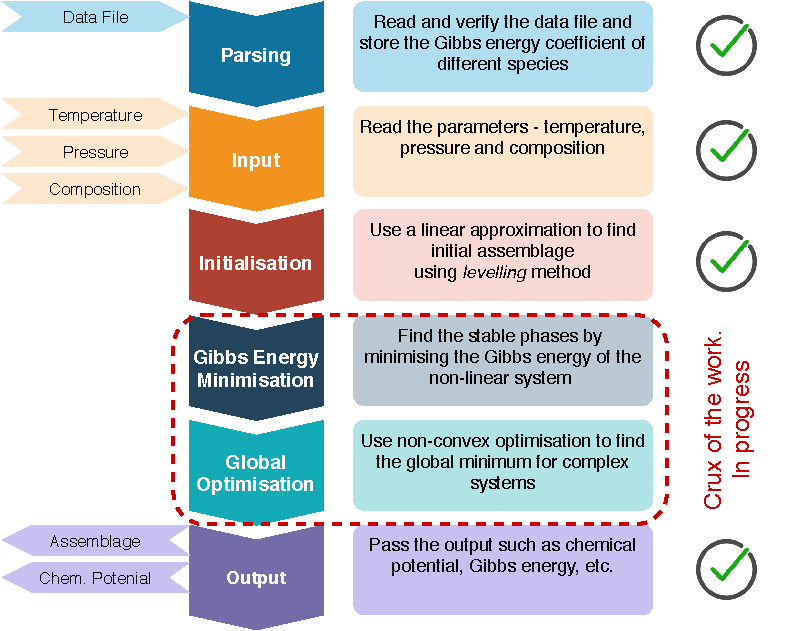
\includegraphics[height=0.65\paperheight]{Figures/YJ_Progress.pdf}
		\end{center}
	\end{figure}
}

\frame{
	\frametitle{Demonstration Problem}
	\only<1>{
	\begin{itemize}
	\item<1> Initial focus on Ni alloys interacting with molten \ce{LiF2 - KF} salts.
	\end{itemize}
	\begin{figure}[htbp]
		\begin{center}
		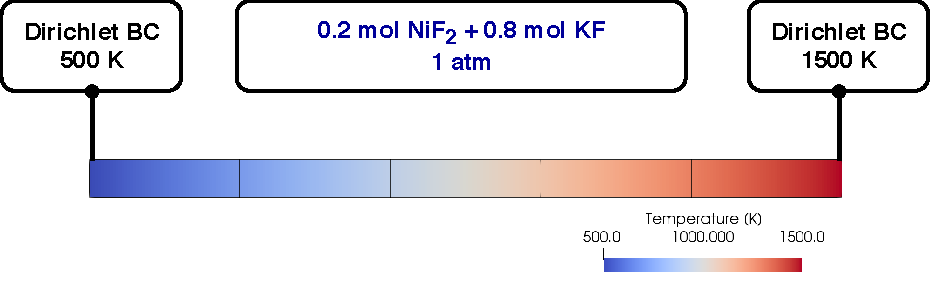
\includegraphics[width=0.85\textwidth]{Figures/Demo_prob.pdf}
		\end{center}
	\end{figure}}
	
	\only<2>{
	\begin{figure}[htbp]
		\begin{center}
		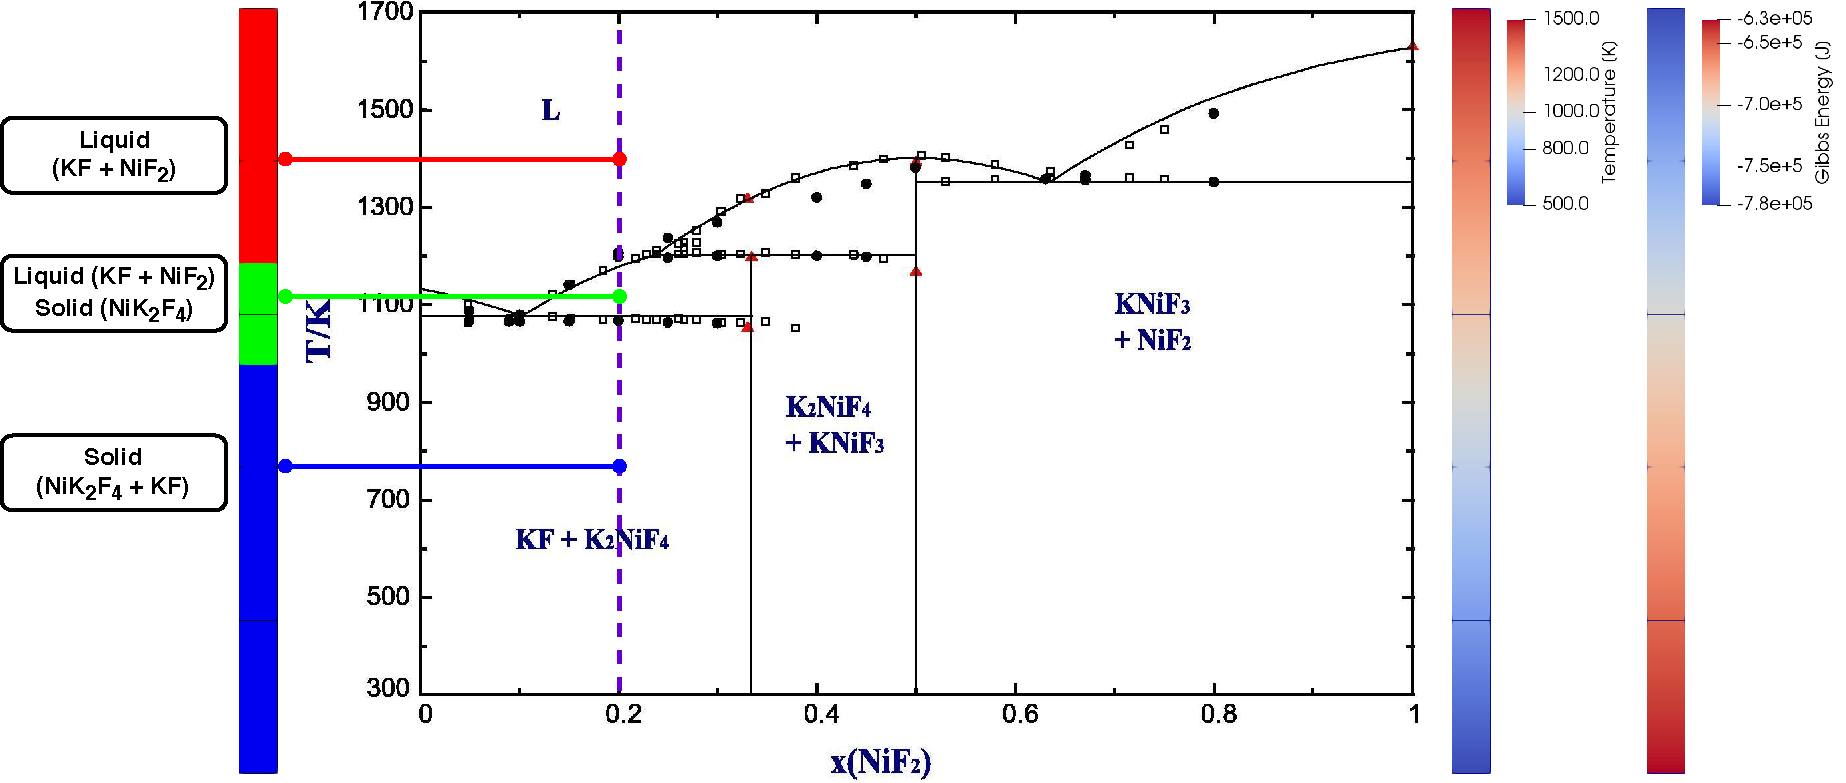
\includegraphics[width=0.85\paperwidth]{Figures/Results.pdf}
		\end{center}
	\end{figure}}
}

\subsection[Timeline]{Timeline}

\frame{
	\frametitle{Timeline - Coursework}
	\tiny
	\begin{table}[!htbp]
		\centering	
  		\begin{tabular}{@{}p{0.6\textwidth} r r@{}}
		\toprule
		\multicolumn{3}{c}{\textbf{Coursework}}\\
		\midrule
		\multicolumn{1}{c}{\textbf{Item}} & \multicolumn{1}{c}{\textbf{Timeline}} & \multicolumn{1}{c}{\textbf{Status}}\\
		\midrule
		MCSC-6010G: Mathematical Modelling & Sep. - Dec. 2018 & Complete\\
		MCSC-6030G: High Performance Computing & Sep. - Dec. 2018 & Complete\\
		NUCL-6005G: Computational Thermodynamics [PhD level elective] & Sep. - Dec. 2018 & Complete\\
		MCSC-6020G: Numerical Analysis & Sep. - Dec. 2019 & Complete\\
		\bottomrule
      		\end{tabular}
	\end{table}
}

\frame{
	\frametitle{Timeline - Research}
	\tiny
	\begin{table}[!htbp]
		\centering	
  		\begin{tabular}{@{}p{0.6\textwidth} r r@{}}
		\toprule
		\multicolumn{3}{c}{\textbf{Research}}\\
		\midrule
		\multicolumn{1}{c}{\textbf{Item}} & \multicolumn{1}{c}{\textbf{Timeline}} & \multicolumn{1}{c}{\textbf{Status}}\\
		\midrule
		Literature review of computational thermodynamics and GEM & Sep. - Dec. 2018 & Complete\\
		Implement data file parsing code & Feb. - Mar. 2019 & Complete\\
		Implement linear solver (levelling) & Apr. - Jun. 2019 & Complete\\
		Implement communication between Yellowjacket and MOOSE & Jul. - Aug. 2019 & Complete\\
		Implement non-linear solver for GEM (homogeneous) & Sep. - Dec. 2019 & In progress\\
		Implement non-linear solver for GEM (heterogeneous) & Jan. - Mar. 2020 & Planned\\
		Demonstration of non-linear solver capabilities & Mar. - May 2020 & Planned\\
		Begin integration of thermodynamic solver with Marmot & Jun. - Aug. 2020 & Planned\\ 
		Comparative study of global optimisation strategies & Sep. - Dec. 2020 & Planned\\
		Implementation of global optimisation algorithm & Jan. - Mar. 2021 & Planned\\
		Demonstration of global optimisation capabilities & Apr. - May 2021 & Planned\\
		Complete integration into MOOSE & Jun. - Aug. 2021 & Planned\\
		Verification and testing & Sep. - Dec. 2021 & Planned\\
		\bottomrule
      		\end{tabular}
	\end{table}
}

\frame{
	\frametitle{Excess Mixing Models}
	\begin{itemize}
		\item {\textbf{Regular Substitutional Models}}
		\begin{itemize}
			\item \textbf{Kohler-Toop Interpolation}
			\begin{equation*}
				g_{\lambda}^{ex} = \sum_{z=1}^Z \phi_z (x_1^{d_1} x_2^{d_2} x_3^{d_3} )
			\end{equation*}
			\item \textbf{Redlich-Kister-Muggiano Interpolation}
			\begin{equation*}
				g_{\lambda}^{ex} = \sum_{z=1}^Z x_j x_k \sum_{\nu = 0} {^\nu}L_{j}
			\end{equation*}
			\end{itemize}
		\item {\textbf{Compound Energy Formalism}}
		\begin{equation*}
			g_{\lambda}^{ex} = 	 \sum_{p=1}^{N_p} \left( \prod_{m=1} y_{m(s)}  \right)   \sum_{z=0}^{N_z} {^zL_{j,k}} (y_j - y_k)^{z}
		\end{equation*} 
		\item {\textbf{Modified Quasichemical Model}}
	\end{itemize}
}

\frame{
	\frametitle{Levelling}
	Mathematically, levelling is achieved through an iterative process that systematically adjusts fixed combinations of phases, subject to the linear equality and inequality mass balance constraints, to progressively minimise the GIbbs energy of the system. At iteration $m+1$, the adjustment to be applied to the relative Gibbs energy of phase $i$ is defined by :
	\begin{equation*} \label{eq:lev_adj}
		\begin{aligned}
			d \hat{G}_i^{m\rightarrow m+1} &= \sum_{j=1}^{C} c_{i,j} d \Gamma_j^{m\rightarrow m+1}\\
			\hat{G}_i^{m+1} &= \hat{G}_i^{m} - d \hat{G}_i^{m\rightarrow m+1}
		\end{aligned}
	\end{equation*}
	where, $c_{i,j}$ denotes the atomic fraction of element $j$ in species $i$ and $d \Gamma_j^{m\rightarrow m+1}$ is the adjustment applied to the chemical potential of element $j$, which in turn is determined by the most stable phases found at iteration $m$. 
}

\frame{
	\frametitle{Levelling}
	\begin{figure}
            \centering
            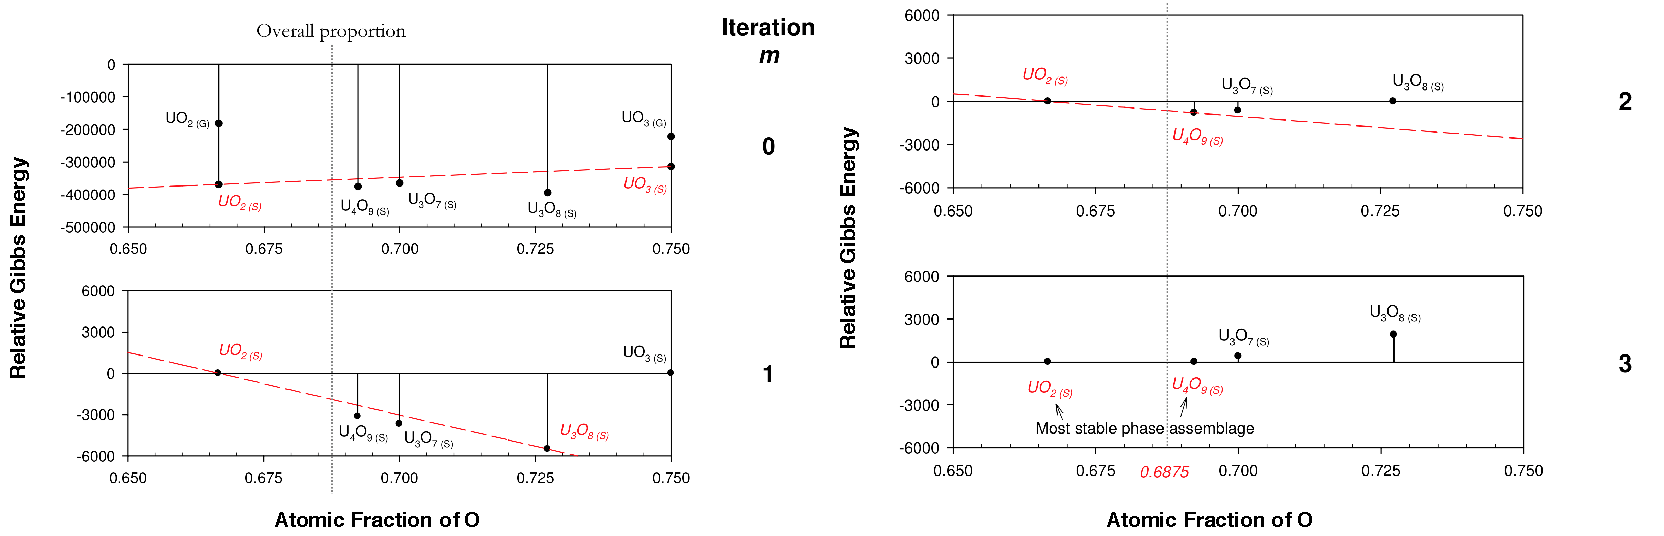
\includegraphics[width=1\linewidth]{Figures/Levelling.pdf}
        \end{figure}
        \blfootnote{M.H.A. Piro, PhD Thesis, RMCC, 2011.}
}


\frame{
	\frametitle{Initialisation - Previous Time Step}
	\begin{figure}[htbp]
		\begin{center}
			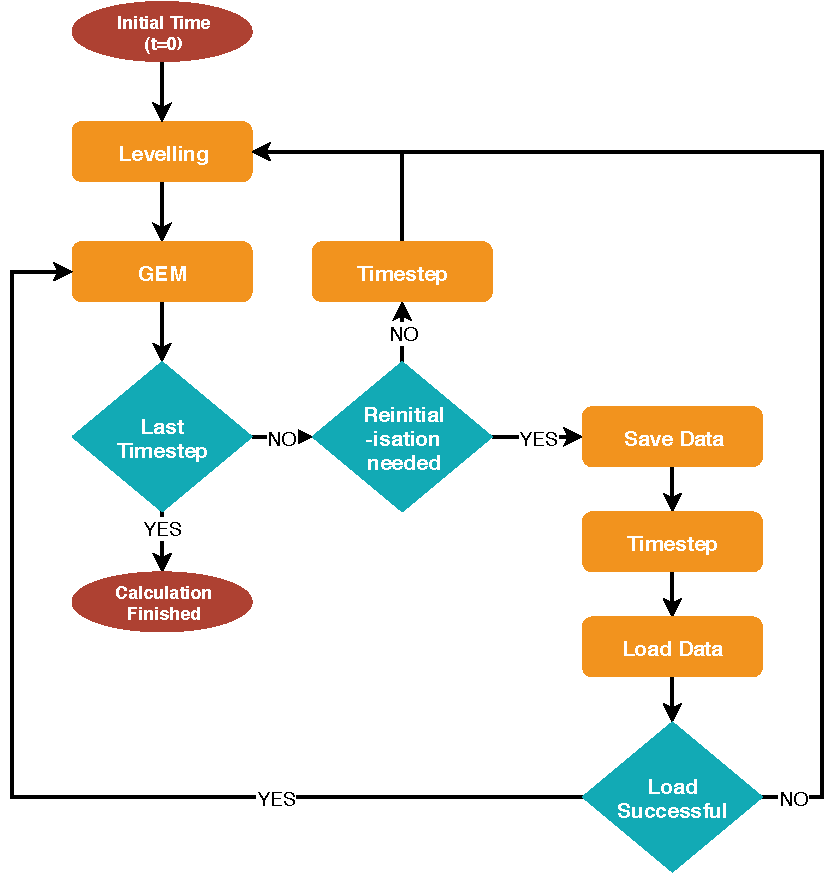
\includegraphics[height=0.75\paperheight]{Figures/Initialisation}
		\end{center}
	\end{figure}
	\blfootnote{Image - Poschmann et al., Technical report, ORNL.}
	
}

\frame{
	\frametitle{Wolfe/Armijo Condition}
	\begin{block}{}
		Each iteration step in the minimisation problem involves approximately solving the subproblem 
		\begin{equation*}
			\min_\alpha f\left(\mathbf{x}^m + \alpha \mathbf{p}^m\right)
		\end{equation*}
	where $\mathbf{x}^m$ is the best estimate at iteration $m$, $\mathbf{p}^m$ denotes the search direction vector and $\alpha$ represents the step size.
	\end{block} 
	
	\begin{exampleblock}{}
		 A step length $\alpha^m$ is said to satisfy the Wolfe conditions, restricted to the direction $\mathbf{p}^m$, if the following two inequalities hold:
	\begin{equation*}
		f\left(\mathbf{x}^m + \alpha^m \mathbf{p}^m\right) \leq f\left(\mathbf{x}^m \right) + c_1 \alpha^m \left(\mathbf{p}^m\right)^T \nabla f\left(\mathbf{x}^m \right)
	\end{equation*}
	\begin{equation*}
		- \left(\mathbf{p}^m\right)^T \nabla f\left(\mathbf{x}^m + \alpha^m \mathbf{p}^m\right) \leq - c_2 \left(\mathbf{p}^m\right)^T \nabla f\left(\mathbf{x}^m \right)
	\end{equation*}
	with $0 < c_1 < c_2 < 1$. The first inequality, known as the Armijo condition ensures that the step length $\alpha^m$ decreases $f$ sufficiently, and the second inequality known as the curvature condition ensures that the slope has been reduced sufficiently.
	\end{exampleblock}
	
}

\frame{
	\frametitle{Particle Swarm Optimisation}
	
	The position vector of the particles at iteration $m$, $\mathbf{x_p^m}$, is updated based on the velocity vector, $\mathbf{v_p^m}$:
	\begin{gather*}
		\mathbf{v_p^m} = \psi \mathbf{v_p^{m-1}} + \phi_p r_p \left(\mathbf{x_p^*} - \mathbf{x_p^m}\right) + \phi_s r_s \left(\mathbf{x_s^*} - \mathbf{x_p^m}\right) \\
		\mathbf{x_p^{m+1}} = \mathbf{x_p^m} + \mathbf{v_p^m}
	\end{gather*}
	where, $x_p^*$ denotes the best known position of a particle (local minima) and $x_s^*$ denotes the best known position of the swarm (global maximum). The first term in the above equation can be interpreted as the inertia term while the second and the third terms act as the driving force towards the local minima and global minimum respectively.}
	
\frame{
	\frametitle{Branch and Bound}
	
	\begin{block}{}
	\begin{enumerate}
		\item \textbf{Branching}: The domain $D$ is partitioned into two or more smaller disjoint domains $D_1,D_2,\dots,$ such that $D = D_1 \cup D_2 \cup \dots$ Thus, the partitioned objective function can be considered a convex approximation of the objective function within the subdomain $D_i$.
		\item \textbf{Bounding}: The upper and lower bound of the objective function are found within a subset of the domain $D$. In the classical Branch and Bound method, a subdomain can be removed from the analysis the lower bound of the objective function in it is greater than the upper bound of the objective function in any other subdomain.
	\end{enumerate}
	\end{block}
	
	\begin{block}{}
	The approach adopted by Piro and Simunovic partitions the domain for each solution phase $\lambda$ into $N_\lambda$ subdomains and the driving force $\pi_\lambda$ is minimised in each subdomain. The Lagrangian function of the driving force of the solution phase $\lambda$ can be defined as follows:
	 \begin{equation*}
	 	L_\lambda = \sum_{i=1}^{N_\lambda} x_{i(\lambda)}\left( \mu_{i(\lambda)} - \sum_{j=1}^{C} \nu_{i,j}\Gamma_j \right) - \pi_{\lambda}\left( \sum_{i=1}^{N_\lambda} x_{i(\lambda)} -  1 \right)
	 \end{equation*}
	 \end{block}	
}


\frame{
	\frametitle{Phase Field Method}
	
	\begin{block}{Cahn-Hilliard Equation}
		\begin{equation}
            		\frac{dc}{dt} = \nabla M\left(c_i\right) \nabla\frac{\delta F}{\delta c_i}
        		\end{equation}
	\end{block}
	
	\begin{exampleblock}{Allen-Cahn Equation}
		\begin{equation}
            		\frac{d\eta_j}{dt} = -L \frac{\delta F}{\delta \eta_j}
        		\end{equation}
        \end{exampleblock}
        
        The primary thermodynamic inputs required to the evolution equations are the Gibbs free energy of the system and chemical potentials of the species as a function of the concentrations of components and the phase order parameters.
}



\frame{
	\frametitle{Continuous Integration Environment for Verification, Enhancement, and Testing (CIVET)}
	\begin{figure}[htbp]
		\begin{center}
			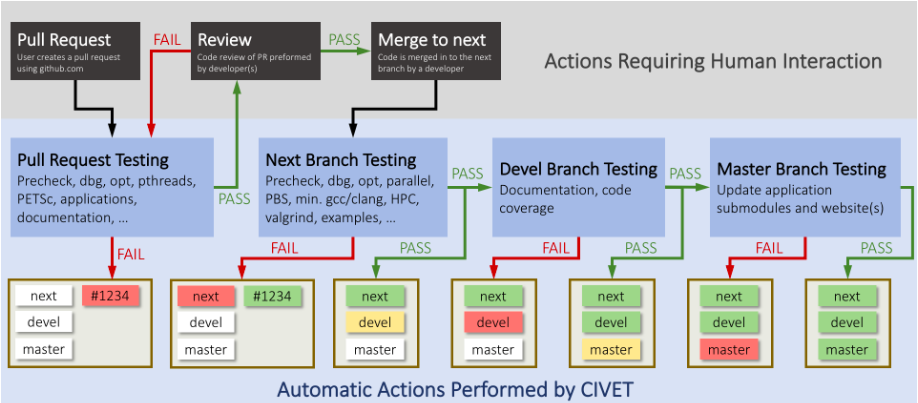
\includegraphics[width=\textwidth]{Figures/CIVET}
		\end{center}
	\end{figure}
	\blfootnote{Image - MOOSE Website \url{https://mooseframework.org/workshop/}}
	
}

\frame{
	\frametitle{Corrosion}
	\begin{figure}[htbp]
\begin{center}
	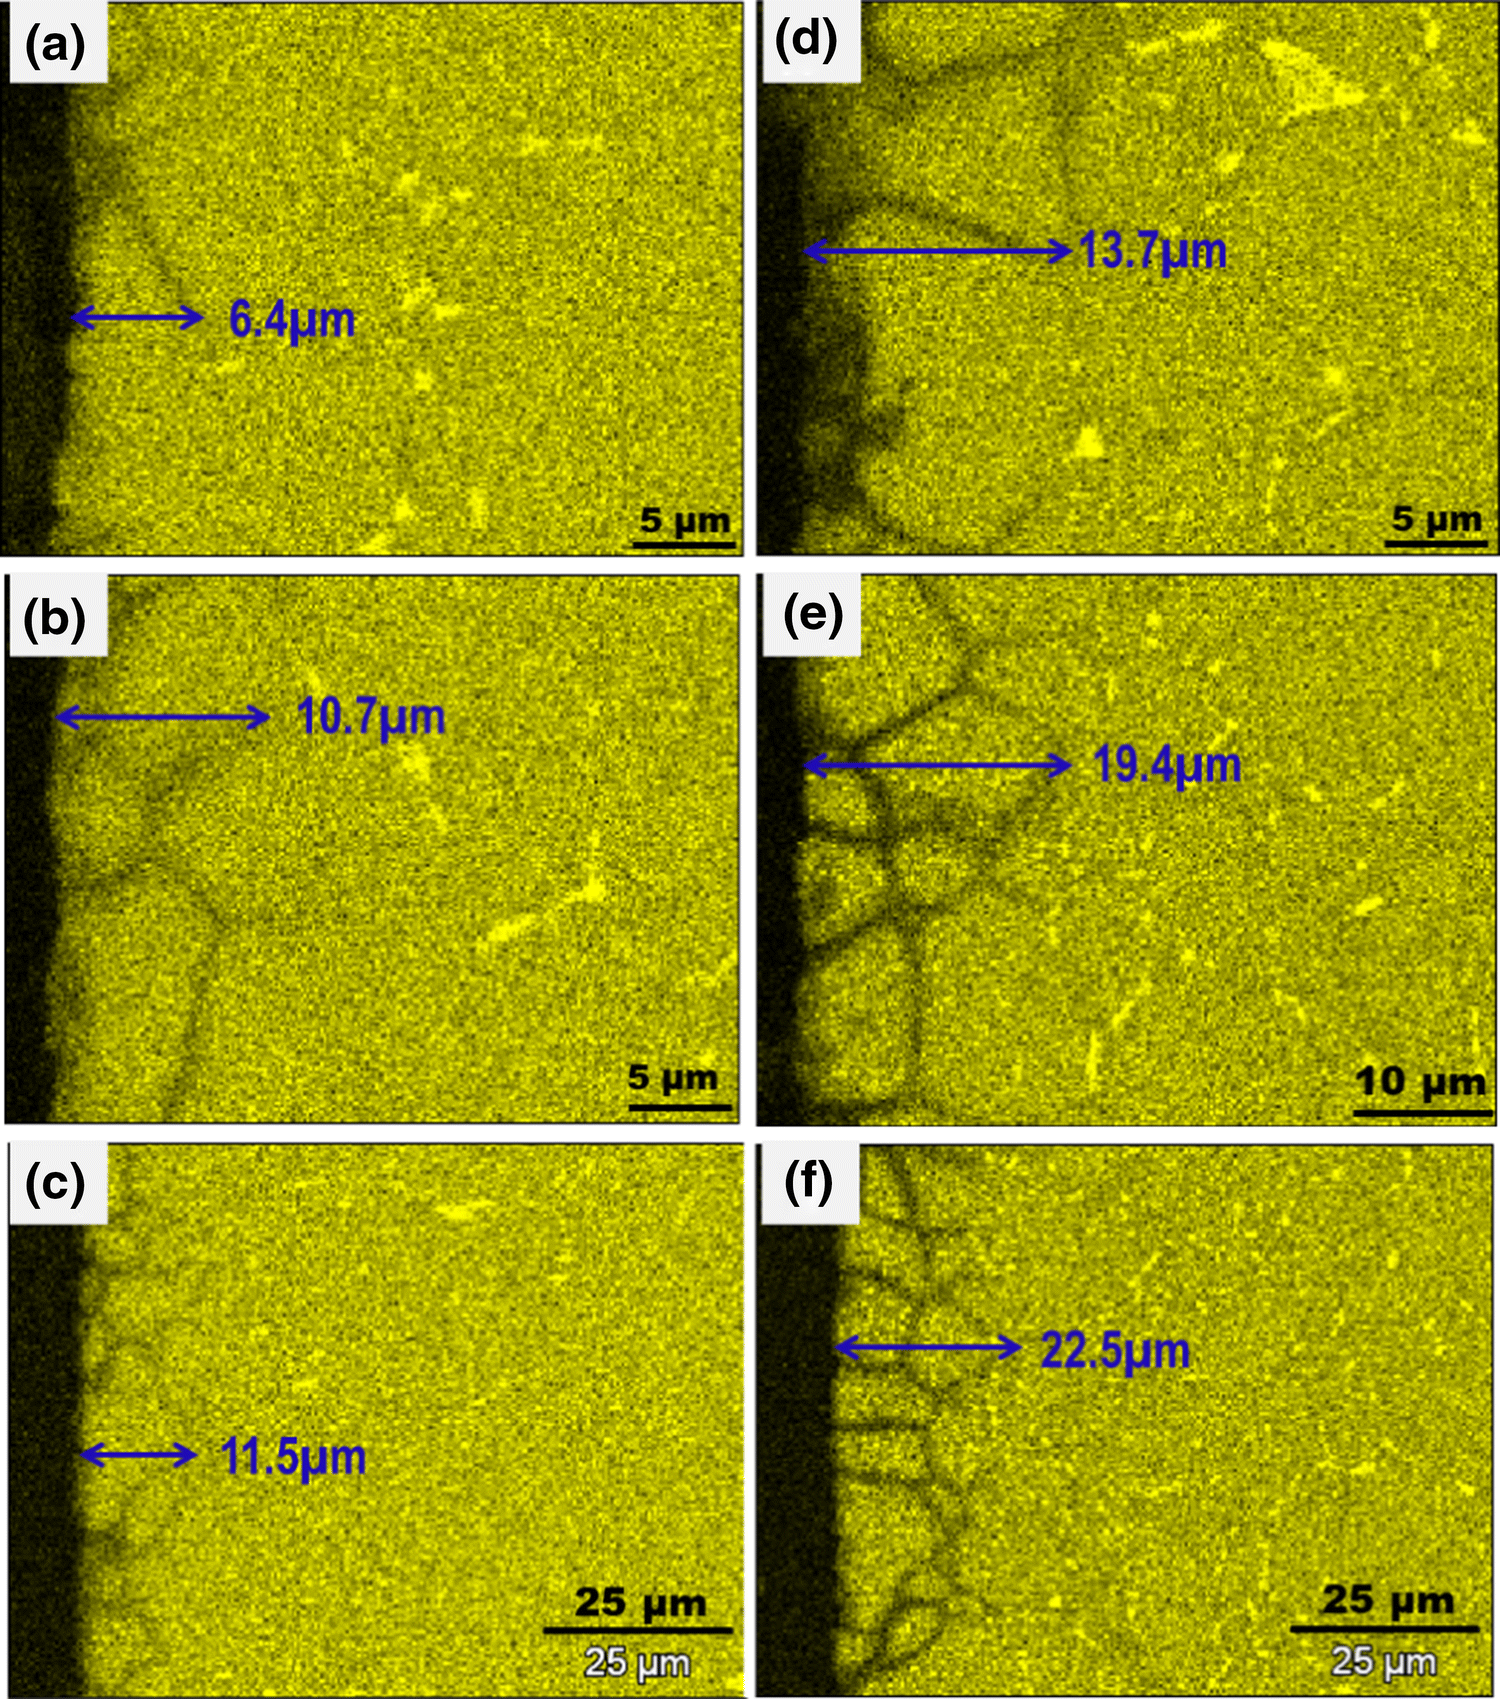
\includegraphics[height=0.6\paperheight]{Figures/Corrosion}
\caption{EDS maps of Cr as a function of depth below the surface of 316 stainless steel samples after corrosion tests: (a–c) tested in 316 stainless steel capsule and (d–f) tested in graphite capsule for 1000 h, 2000 h, and 3000 h, respectively. The maximum Cr depletion distance along grain boundaries is labeled in each EDS Cr map.}
\end{center}
\end{figure}

	\blfootnote{Zheng et al.,  J. Nucl. Mater., 461, 143-150, 2015.}
}



%\begingroup
%\setbeamertemplate{navigation symbols}{}
%{
%\setbeamercolor{background canvas}{bg=}
%
\includepdf{Cover/BackCover.pdf}
%}
%\endgroup

\end{document}
